\chapter{Experimentation}
\label{chap:5_approach}
\section{Overview}
In this chapter we will present in detail the planning and approach we followed to establish the experiments on the application of \tdd for \ess, and provide an initial analysis of the results.

A controlled experiment, the baseline (\textit{Exp1}), followed by its replication (\textit{Exp2}), was conducted with the participation of 9 undergraduate final-year Master's degree and third-year Bachelor's degree Computer Science students enrolled in the \textit{Embedded Systems} course at the University of Salerno, in Italy. Participation in the studies was agreed upon by the students and was voluntary, with the outcome not directly affecting their final mark for the exam; students were however awarded 2 bonus points, in order to encourage their participation.
Before taking part in the first experiment, a set of lectures and training sessions was held with the objective of providing the participants with a common body of knowledge on the topics tackled by the experiments, namely unit testing, test scaffolding, and the \tdd approach.

Afterwards, the participants were partitioned into two groups and tackled the first task of \textit{Exp1}, one group using \tdd, the other using \notdd; this task, \textit{IntelligentOffice} (\textit{IO}) required the implementation of a system responsible for handling various parameters and functionalities inside a smart office, including the detection of workers, handling the lights and monitoring the CO2 levels inside the office.
For the second task, \textit{CleaningRobot} (\textit{CR}), the approach followed by the two groups was inverted, namely the group that implemented the first task using \tdd switched to \notdd and vice versa. This task concerned the development of an \es to manage a small cleaning robot which had to move in a room to clean dust, while avoiding obstacles along the way.
After each task of \textit{Exp1} the participants were asked to fill a questionnaire to express their feelings about the experience.

For (\textit{Exp2}), the participants had to develop an additional \es, this time at home on their own (\ie not under our supervision in a laboratory of the university), before submitting their implementation and deploying it on a real hardware platform, a \textit{Raspberry Pi Model 4}, and using real sensors and actuators. This task, \textit{SmartHome} (\textit{SH}), was focused on the implementation of an intelligent system which allowed for handling light, temperature, and gas levels inside a room.
Since \textit{Exp2} was only made up of this task, the students were randomly assigned one of the two approaches (\ie \tdd or \notdd) upon receiving the instructions for implementing this \es.
The students were given a deadline to implement the task, and were asked to book a time slot, during which they would have deployed their implementation on hardware and would have tested it in real time by observing the behavior of the sensors and actuators; moreover, each participant was individually interviewed after the hardware deployment step, in order to gather qualitative data regarding their feedback on the experiments.

Following the three tasks, we extracted the statistical values for a set of predefined dependent variables by running the acceptance test suite we prepared for each task on the implementations delivered by the participants. These values, as well as the submitted post-questionnaires and final interview, were our primary subject of analysis to answer the established research questions on the impact of \tdd on the external quality, productivity, and number of written test cases of the developers' implementations when tackling \ess.

Overall, this experimental study aims to contribute to the body of knowledge in the field of empirical software engineering by providing new insights and understanding into the application of \tdd for \es development. Furthermore, it has both research and educational goals: on one hand, we conceived the study to answer our RQs; on the other, the study allowed the participants (students) to gain practical experience with \tdd applied to \ess. As for the educational goal, \tdd is a development approach widely used in several contexts \cite{DBLP:conf/esem/RomanoZBPS22}, and it seems to be promising in the development of \ess too \cite{TDDEC}.

Although the preliminary and exploratory nature of our investigation, it has the merit to study for the first time the application of \tdd in a new development context, namely that of \ess; therefore, our results can have several practical implications, for both lecturers and researchers. For example, they could provide initial evidence on the application of \tdd to the development of \ess as to justify future research on this matter and/or promote or discourage its adoption in an industrial setting.


\newpage
\section{Research questions}
Following the main research question presented in the introduction chapter of the thesis, we defined the main goal of this study by applying the Goal/Question/Metrics (GQM) template \cite{GQM}.
According to this template, for an organization to measure purposefully it must first specify the goals for itself and its projects, then it must trace those goals to the data that are intended to define those goals operationally, and finally provide a framework for interpreting the data with respect to the stated goals.
We identify our goal as follows:

\begin{framed}
\noindent
\textbf{Analyze} the use of \tdd 
\textbf{for the purpose of} evaluating its effects in the development of \ess
\textbf{with respect to} the external quality of the implemented solution, the developers' productivity, and the number of written test cases
\textbf{from the point of} view of the researcher and lecturer 
\textbf{in the context of} an \ess course involving second year Master's degree students in Computer Science.
\end{framed}

\noindent According to this objective, the following research questions were defined:
\begin{itemize}
    \item \textbf{RQ1.} Does the use of \tdd impact the quality of the developed \es? And if so, to what extent?

    \noindent\textit{Aim}: The answer to this RQ has practical implications, especially within the Agile community: for example, in case the use of \tdd positively affects the quality of \ess developed within implementation tasks, it would mean that it is the case to teach this development approach in academic contexts, with the ultimate goal of facilitating the adoption of this Agile technique in the industry. 
    That is, if the newcomers of the working market are familiar with \tdd (because they learned and experienced it in the academic context), and it is shown that it produces \ess with improved quality, then the software industry could be encouraged to migrate their development from \notdd to \tdd.

    \item \textbf{RQ2.} Does the use of \tdd increase developers' productivity when developing \ess? And if so, to what extent?

    \noindent\textit{Aim}: A positive answer to this RQ has practical implications, since it would help us to further improve our body of knowledge in the context of \tdd applied to the development of \ess. For example, some software companies operating in the context of the development of \ess could be encouraged to use \tdd in case: \textit{(i)} there is evidence that this approach improves productivity and \textit{(ii)} developers are familiar with this approach before being hired (\eg \tdd has been learned at university).

    \item \textbf{RQ3.} Does the use of \tdd increase the number of test cases written by developers when developing \ess? And if so, to what extent?

    \noindent\textit{Aim}: If the adoption of \tdd were to result in a higher number of written test cases when developing \ess, using this approach would be beneficial to the industry. Not only more test cases would potentially cover more of the implemented source code, thus increasing reliability; additionally, the fact that tests are written as the first thing when using \tdd, a higher number of them would provide more documentation for developers and new contributors to the system, especially for those aspects of \ess that concern lower-level details, such as hardware interaction, and are generally harder to test. Finally, more tests would open up more refactoring opportunities when using \tdd; this could help with the optimization steps commonly performed in many \ess.
\end{itemize}




\section{Participants}
The participants for both \textit{Exp1} and \textit{Exp2} were Computer Science students at the University of Salerno, in Italy; they were a mix of second-year Master's degree students in Salerno, and students visiting the university by means of the Erasmus program. Both groups were enrolled in the \textit{Embedded Systems} course at the University of Salerno, however not all students had a strong Computer Science background, and among those taking the course, 9 participated. 

Participating in the studies was voluntary: the students were informed that \textit{(i)} any gathered data would be treated anonymously and shared for research purposes only; \textit{(ii)} they could drop out of the study at any time if they wished to do so, and \textit{(iii)} they could achieve the highest mark in the course even if they did not participate. Finally, as an incentive to encourage participation, those who took part in the studies were rewarded with 2 bonus points in their final mark for the course, in line with Carver \etal's advice \cite{DBLP:conf/metrics/CarverJMS03}.

Before \textit{Exp1} took place, we collected some information on the participants' knowledge and experience with general programming and testing concepts, in order to get a general idea of their personal preparation before the studies. To this end, the participants were asked to fill out a form in which they had to rate their experience using an interval-scale questions system (where 1 means “very inexperienced” and 5 means “very experienced”). All the participants had programming experience and most of them rated such an experience as 3 out of 5 on the scale. 
As for testing, the participants were mostly not experienced with unit testing, since most of them chose 1 or 2 on the scale to represent their unit-testing level of experience; finally, three students had heard about \tdd, from another university course, but none had had a practical experience with this technique before the study.

The participants for the experiments were later asked to carry out their task by either using \tdd or \notdd (\ie any approach they preferred, except for \tdd) depending on the group they were partitioned in, and on the period the task took place in. 





\section{Experimental tasks design}
The experimental objects designed for the studies are three code katas, \ie programming exercises aimed at practicing a technique or a programming language: in this case the design of a small \es, which would take around 2 hours to implement. 
All three tasks were designed according to a target platform, a \textit{Raspberry Pi Model 4}, and using the \textit{Python} programming language. As for why this environment was chosen, compared to other programming languages and platforms typically used for \ess or \iot projects (\eg \textit{Arduino} with \textit{C++}), in our opinion designing the tasks with a higher level language such as \textit{Python} - which is still employed for \ess (either in its standard form or in its \textit{MicroPython} variant), as well as for Web and Enterprise applications, as reported by IEEE Spectrum \cite{IEEESpectrum} - allowed us to focus more on the implementation and logic details than we would have done by designing the tasks orbiting around lower level language features and mechanisms.
Furthermore, if we also take into account that some participants had a limited, mostly theoretical, knowledge of \ess prior to the course's end, we think that introducing these practical concepts with \textit{Python} made it easier for them to get a grasp on the main implementation concepts for \ess. Finally, participants relied on the \textit{PyCharm IDE} to implement all three tasks, with the native \texttt{unittest} package as the testing library.

The target platform was considered even during the design of the two tasks of \textit{Exp1}, which in the end did not have to be effectively deployed on hardware; this was done in order to make the mocked implementations developed by the participants resemble as closely as possible the embedded implementations, in line with the approach proposed by Grenning \cite{TDDEC}. The main mocked component utilized was a facade for the \textit{Raspberry Pi}'s General Purpose Input/Output (GPIO) library, available as open source software on GitHub \cite{GPIOMock}. Other mocked components included third party libraries for some individual sensors and actuators, like for the \textit{DHT11} temperature and humidity sensor.
For \textit{Exp2}, another factor that influenced the design of the code kata was the availability of the hardware at the university, including sensors and actuators, as well as how hard/practical these would have been to test in real time; for example, testing a gas sensor by actually releasing gas close to it for extended periods of times could be dangerous. For some sensors, on the other hand, this was not a concern since it was possible to manually trigger them by rotating an on-board potentiometer, effectively lowering or increasing the detection threshold for their respective measurements.
The task developed for \textit{Exp2} was later deployed and tested inside a laboratory at the University of Salerno: each participant had their project uploaded on a \textit{Raspberry Pi model 4} board and assisted as we ran a small acceptance test suite in real time and logged the results (\ie which test cases passed and which failed). 

For \textit{Exp1}, the experimental tasks were:
\begin{itemize}
    \item \textbf{\textit{IntelligentOffice}} (\textbf{\textit{IO}}): task revolving around the implementation of a smart system to manage an office, by using different sensors and actuators to handle various aspects inside it. The system was responsible for detecting the presence of workers in four quadrants of the office by using infrared (IR) distance sensors, manage the light level in the room with a smart light bulb, a photoresistor (or Light Dependent Resistor, LDR), and a set of blinds controlled by a servo motor; the motor opened/closed the blinds based on the time of day and day of week measured by a Real Time Clock (RTC) module. Finally, the system would monitor the CO2 levels inside the office, with the possibility of triggering an air vent system to balance them by expelling the air outside.

    \item \textbf{\textit{CleaningRobot}} (\textbf{\textit{CR}}): as the name suggests, this task required participants to implement an \es to manage a small cleaning robot. This system received command strings from an external management unit, and had to move/rotate the robot inside the room accordingly, using two Direct Current (DC) motors, one for the wheels, and one for the robot itself. Besides this, the robot had to be able to detect obstacles in front of it by using an IR distance sensor, and had to communicate its position and the last encountered obstacle back to the remote management system after performing an action. Finally, an Intelligent Battery Sensor (IBS) was used to check the charge left of the internal battery of the robot, and a LED was turned on to signal the need for a recharge; similarly, the cleaning system of the robot would be turned on/off according to the measured remaining battery level.
\end{itemize}

As for \textit{Exp2}, the replication experiment, the \es to implement was the following:
\begin{itemize}
    \item \textbf{\textit{SmartHome}} (\textbf{\textit{SH}}): this final task concerned the development of a system which allowed the handling of light, temperature, and gas levels inside a room. By using an IR distance sensor, a photoresistor and a smart light bulb, the system managed the light level inside the room to avoid wastefully turning the light on when the user was not in the room or when it was already bright enough due to natural light. Furthermore, two temperature sensors, one on the inside and one on the outside of the room were used to collect measurements, based on which a servo motor opened or closed a window in the room. Finally, the system was also equipped with an air quality sensor to measure the gas levels inside the room; based on these measurements, in case of high amounts of gas particles detected in the air, an active buzzer would trigger an alarm to notify the user.
\end{itemize}

Further details on the experimental objects, including the list of user stories, sensors and actuators employed, and other information, are provided as an appendix to this thesis (\ref{appendix:A_IntelligengOffice}, \ref{appendix:B_CleaningRobot}, \ref{appendix:C_SmartHome}).

The material provided to the participants for each task included: \textit{(i)} a document containing the description of the task, made up of a high level description of the purpose of the system, instructions on the development approach (\ie \tdd or \notdd), and the list of user stories to implement, with each detailing the corresponding class/method to modify in the source code; and \textit{(ii)} a link to project template for the \textit{PyCharm IDE} that the participants had to import in their environment (\ie by either forking/cloning the corresponding GitHub repository or by downloading a zip file); this template contained method stubs (\ie empty methods exposing the expected API signatures), utility functions, mocked libraries for the GPIO features and other components, as well as an example empty \texttt{unittest} test class.

For each of these tasks, we prepared a corresponding acceptance test suite, as a mean to evaluate the implementations delivered by participants, and extract the metrics on which to base our empirical assessment.


\section{Study design}
The \textit{Embedded Systems} course, during which the study was conducted, started in September 2022 and covered the following topics: modeling and design of an \es, state machines, sensors and actuators, embedded processors, memory architectures, embedded security and privacy concepts, embedded operating systems and scheduling, and \ess testing techniques.

As the survey pre-\textit{Exp1} highlighted, few students had unit testing experience, and almost no participants ha dealt with \tdd up to that point: for this reason, both topics were covered through a series of frontal lectures and exercise/homework sessions in the weeks preceding the \textit{Exp1}. All the participants attended these lectures and training sessions during which they had some theoretical and hands-on experiences with the main topics they would encounter during the future experimental tasks. The overall schedule for training sessions and studies was as follows:
\begin{itemize}
    \item \textbf{Day1.} Frontal lecture - Introduction on unit testing and its guidelines - Interactive exercise on unit testing.
    \item \textbf{Day2.} Frontal lecture - Test scaffolding and \textit{Raspberry Pi}'s GPIO library - Interactive exercise on test scaffolding.
    \item \textbf{Day3.} Frontal lecture - Introduction to \tdd - Interactive exercise on \tdd.
    \item \textbf{Day4.} Training task - \tdd exercise and homework with the same structure as the future experimental task (\ie project template, a set of user stories, and 2 hours deadline).
    \item \textbf{Day6.} First task for \textit{Exp1} (\textit{IO}).
    \item \textbf{Day7.} Second task for \textit{Exp1} (\textit{CR}).
    \item \textbf{Day8.} Start date for the task relative to \textit{Exp2} (\textit{SH}).
\end{itemize}


The first task, \textit{IO} took place on Tuesday, December $6^{th}$ 2022, while the second, \textit{CR} took place on Tuesday, December $13^{th}$ 2022; both tasks required around 2 hours to be implemented by the participants. Finally, the start date for \textit{Exp2} (\ie the date when we sent out the documentation to the students) was December $19^{th}$ 2022, and the participants had to deliver their implementation by January $8^{th}$ 2023.

The design of \textit{Exp1} is an ABBA crossover \cite{DBLP:journals/tse/VegasAJ16}; it is a kind of \textit{within-participants} design where each participant receives both treatments (\ie \textit{A} and \textit{B} or, in our case, \tdd and \notdd). In ABBA crossover designs, there are two sequences (\ie \textit{G1} and \textit{G2}), defined as the order with which the treatments are administered to the participants, and two periods (\ie \textit{P1} and \textit{P2}), defined as the times at which each treatment is administered; the experimental groups correspond to the sequences. Also, to mitigate learning effects, each period is paired with a
different experimental task.

For the first period \textit{P1}, the group \textit{G1} was assigned the \tdd version of the first task, \textit{IO}, while the group \textit{G2} was assigned the \notdd version; on the other hand, during period \textit{P2}, the group \textit{G1} was assigned the \notdd version of the second task, \textit{CR}, while the group \textit{G2} was assigned the \tdd version.
Therefore, at the end of \textit{Exp1}, every participant had tackled each experimental object only once.
As for \textit{Exp2}, the group structure remained the same, however each participant was randomly assigned the \tdd or \notdd version of the third and final experimental task, \textit{SH}; specifically, 5 students ended up in the \tdd group, while 4 formed the \notdd group. As a result, the design of this study is \textit{one-factor-with-two-treatments} \cite{DBLP:books/sp/WohlinRHOR00}, a kind of \textit{between-participants} design.

After each period of \textit{Exp1}, participants were asked to fill out an online questionnaire, with the purpose of describing their general experience with the implementation of the task, focusing on their perceived complexity and testing approach. 
The structure of the post-questionnaires was made up of three interval-scale questions, and a variable number of open-ended questions, two for the \tdd group and three for the \notdd group, with the latter having an additional question, as the first open-ended one, asking to provide information about the chosen approach for testing. Furthermore, the post-questionnaire presented at the end of period \textit{P2} for \textit{Exp1} contained an additional open-ended question: here, participants had to provide their feelings towards both testing practices, \tdd and \notdd, and compare them based on the two encountered tasks. More specifically, the interval-scale questions were:

\begin{itemize}
    \item \textbf{Q1.} Regarding the comprehensibility of the provided user stories, I have found them: (Very unclear $|$ Unclear $|$ Neither clear nor unclear $|$ Clear $|$ Very clear).
    \item \textbf{Q2.} I have found the development task: (Very difficult $|$ Difficult $|$ Neither easy nor difficult $|$ Easy $|$ Very easy).
    \item \textbf{Q3.} Applying this testing approach (\ie \tdd or \notdd) to accomplish the development task has been: (Very difficult $|$ Difficult $|$ Neither easy nor difficult $|$ Easy $|$ Very easy).
\end{itemize}

\noindent As for the open-ended questions, these were:
\begin{itemize}
    \item (\textbf{\notdd only}) Describe the \notdd approach you have followed to accomplish the development task.
    \item Provide your feelings (both positive and negative) about the testing approach you used (\ie \tdd or \notdd).
    \item Provide your feelings (both positive and negative) about the development task.
    \item (\textbf{Task 2 only}) After applying the testing approach (\ie \tdd or \notdd) in the last exercise, do you have any thoughts on the differences between the two and your preference for using one over the other?
\end{itemize}

\noindent Finally, no formal questionnaire was provided for the replication study; however, after the hardware deployment and testing steps, each participant was individually interviewed about their overall experience with the studies; the structure of the final interview had a predefined script, as suggested by King \cite{King:2004}. The topics covered by the interview were:
\begin{enumerate}
    \item Provide your feelings (both positive and negative) about the final development project, (\eg development pipeline, used technologies).
    \item Provide your feelings (both positive and negative) about the development approach (\ie \tdd or \notdd) used to accomplish the final development project:
        \begin{itemize}
            \item \tdd: did you perform any refactoring? 
            \item \notdd: did you test your implementation at all? If so, which approach did you use?
        \end{itemize}
    \item Provide your feelings about the overall training experience (seminars, exercises, and homework on \tdd and \notdd, experiments, and final task):
        \begin{itemize}
            \item Positive and negative points and challenges encountered when applying TDD.
            \item What can be done to improve the application of TDD in the development of \ess?
            \item Provide a discussion on \tdd vs. \notdd in the development of \ess.
        \end{itemize}
\end{enumerate}

The answer for both the post-questionnaires and the final interviews, as well as their thematic analyses, are available as an appendix to this thesis (\ref{appendix:D_Thematic_Analysis_Baseline}, \ref{appendix:E_Thematic_Analysis_Replication}).



\section{Independent and dependent variables}
The participants were asked to carry out each task by using either \tdd or the approach they preferred (\notdd), therefore one of the independent variables considered is \textbf{\textit{Approach}}, a nominal variable assuming two values, \tdd and \notdd. The data was collected over two periods for the controlled baseline study (\textit{Exp1}), and over an additional period for the non-controlled replication study (\textit{Exp2}), so a second independent variable is \textbf{\textit{Period}}, assuming the values $P1$, $P2$, and $P3$. During the three periods both approaches (\tdd or \notdd) were applied. Finally, since the participants were split into two groups, the last independent variable is \textbf{\textit{Group}}, which can assume the values \textit{G1} and \textit{G2}.

As for the dependent variables considered in the experiments, these are: \textbf{\textit{QLTY}}, \textbf{\textit{PROD}}, \textbf{\textit{TEST}}, \textbf{\textit{CYC}}, \textbf{\textit{COG}}, \textbf{\textit{LOC}}.
The variables $QLTY$, $PROD$ and $TEST$ have been used in previous empirical studies on \noess \cite{DBLP:journals/tse/ErdogmusMT05}, \cite{DBLP:journals/tse/FucciETOJ17}, \cite{DBLP:conf/esem/Fucci0BCSTJ18}, \cite{DBLP:journals/ese/TosunDFVTESOTJJ17}. 
As for the other variables (\ie $CYC$, $COG$, and $LOC$), while they could just be used to assess constructs regarding code complexity, they can also be leveraged to further assess the quality of a software solution, since they have an impact on external attributes, such as efficiency, reliability, and maintainability.

QLTY quantifies the external quality of the solution a participant implemented. It is formally defined as follows: 
\[
    QLTY = \frac{\sum_{i=1}^{\#TUS} QLTY_i}{\#TUS} * 100 
\]
where $\#TUS$ is the number of user stories a participant tackled, while $QLTY_i$ is the external quality of the $i$-th tackled user story; to determine whether a user story was tackled or not, the asserts in the test suite corresponding to the story were checked: if at least one assert in the test suite for the story passed, than the story was considered as tackled. $\#TUS$ is formally defined as follows:
\[
    \#TUS = \sum_{i=1}^{n} 
        \begin{cases}
            1 & \text{$\#ASSERT_i(PASS) > 0$}\\
                0 & \text{otherwise}
        \end{cases}
\]
Finally, the quality of the $i$-th user story (\ie $QLTY_i$) is defined as the ratio of asserts passed for the acceptance suite of the $i$-th user story over the total number of asserts in the acceptance suite for the same story. More formally:
\[
    QLTY_i = \frac{\#ASSERT_i(PASS)}{\#ASSERT_i(ALL)}
\]
As a result, the $QLTY$ measure deliberately excludes unattempted tasks and tasks with zero success; therefore, it represents a local measure of external quality calculated over the subset of user stories that the subject attempted. $QLTY$ is a ratio measure in the range $[0, 100]$.

The PROD variable estimates the productivity of the solution implemented by a participant. It is computed as follows:
\[
    PROD = \frac{\#ASSERT(PASS)}{\#ASSERT(ALL)} * 100
\]
where $ASSERT(PASS)$ is the total number of asserts that have passed, by considering all acceptance test suites, while $ASSERT(ALL)$ refers to the total number of asserts in the acceptance suites. The $PROD$ variable can assume values between 0 and 100, where a value close to 0 indicates low productivity in the implemented solution, while a value close to 1 refers to high productivity.

The $TEST$ variable quantifies the number of unit tests a participant wrote in their implementation. It is defined as the number of assert statements in the test suite written by the participant; this variable ranges from 0 to $\infty$.

As for the additional three dependent variables, these were computed using SonarQube, an open-source platform for continuous inspection and static analysis of code \cite{SonarQube}; these variables provide additional insight regarding the quality in the implemented software solution, mostly in terms of how hard the production code is to comprehend and therefore maintain. 

They can be defined as follows:
\textbf{$CYC$} refers to the cyclomatic complexity metric of the implemented solution; it is a value used to determine the stability and level of confidence in a program, and it measures the number of linearly-independent paths inside a code module; a program with a lower cyclomatic complexity is generally easier to understand and less ``risky" to modify; the variable can also be used as an estimate on how difficult the code will be to cover/test.

\textbf{$COG$} is the cognitive complexity of the solution; it is a measurement of how difficult a program module is to intuitively understand. A method's cognitive complexity is based on a few rules \cite{CognitiveComplexity}:
\begin{enumerate}
    \item Code is not considered more complex when it uses shorthand syntax that the language provides for collapsing multiple statements into one.
    \item Code is considered more complex for each break in the linear flow of the code.
    \item Code is considered more complex when flow breaking structures are nested.
\end{enumerate}

Finally, $LOC$ is the total number of lines of code written by the participant; it's defined as the sum of the individual lines of code in both the production code source files and the test code source files.

For both $CYC$ and $COG$ we only considered the production code, since there was no noticeable difference, besides one outlier, between the same metrics in the test files of the participants.

Generally speaking, the higher the values of $CYC$, $COG$, and $LOC$, the worse it is: software with high cyclomatic and cognitive complexity is more difficult to understand, maintain, and extend, and is more prone to errors and bugs. It is good practice to keep these complexities (as well as the number of lines of code, although to a lesser extent) as low as possible for easier maintenance and extensibility.





\section{Analysis methods}
\subsection{Individual analysis}
As a first way to examine the distributions of the dependent variables, we computed some descriptive statistics, for each of them. We organize this information inside a set of tables for each experimental task. Moreover, in order to provide a graphical representation of the data and to summarize the distributions, we employ box plot charts.

The information that can be extracted form a box plot chart includes:
\begin{itemize}
    \item \textbf{Minimum value}: the lowest value, excluding outliers (shown at the end of the lower whisker).
    \item \textbf{Maximum value}: the highest score, excluding outliers (shown at the end of the upper whisker).
    \item \textbf{Median}: marks the mid-point of the data and is shown by the line that divides the box into two parts. Half the values are greater than or equal to this value and half are less than this value.
    \item \textbf{Inter-quartile range}: the middle “box” represents the middle 50\% of values for the group: the range of values from lower to upper quartile is referred to as the inter-quartile range; the middle 50\% of scores fall within the inter-quartile range.
    \item \textbf{Upper quartile}: 75\% of the scores fall below the upper quartile.
    \item \textbf{Lower quartile}: 25\% of scores fall below the lower quartile.
    \item \textbf{Whiskers}: the upper and lower ``whiskers" represent scores outside the middle 50\% (\ie the lower 25\% of scores and the upper 25\% of scores).
    \item \textbf{Outliers}: observations that are numerically distant from the rest of the data. They are defined as data points that are located outside the whiskers of the box plot, and are represented by a dot.
\end{itemize}



\subsection{Aggregate analysis}
Meta-analysis is a statistical method used to combine the results of multiple studies in order to obtain a more precise estimate of the effect of the treatment/intervention; its goal is to increase the power of the analysis and to provide a more robust estimate of the treatment's effects.
There are different methods used to conduct a meta-analysis, but generally, the process involves identifying the relevant studies, extracting data from them, and then analyzing this data by employing statistical techniques. 
In our case, after considering the mean, standard deviation, and number of participants for each development approach in \textit{Exp1} and \textit{Exp2}, we made use of the Standard Mean Difference (SMD) as the measure of the effect size for the meta-analysis: this value represents the difference between the two groups' mean values, standardized by dividing the difference by the standard deviation; SMD can be used to determine the overall effect size when comparing the results of the different studies. More formally, it is computed as follows:
\[
    \theta = \frac{\mu_1 - \mu_2}{\sigma}
\]
Where $\mu_1$ and $\mu_2$ represent the two means, and $\sigma$ refers to the standard deviation, used to measure the amount of variation or dispersion of a set of values.
We computed the SMD as \textit{Hedges' (adjusted) g.}; to obtain joint SMDs (one for each dependent variable), we leveraged random-effects meta-analysis models.
\noindent Based on the guidelines proposed by Cohen \cite{Cohen:1992}, the SMD can be interpreted as: \textit{negligible}, if $|\text{SMD}| <$ 0.2; \textit{small}, if 0.2 $\le |\text{SMD}| <$ 0.5; \textit{medium}, if 0.5 $\le |\text{SMD}| <$ 0.8; or \textit{large}, otherwise \cite{DBLP:conf/esem/RomanoZBPS22}.

\ \\ \
A forest plot is a common way to visually present the results of a meta-analysis: it is a representation of the effect estimates and their corresponding confidence intervals for each study included in the meta-analysis. The forest plot is divided into two parts: the left side shows the individual study results and the right side shows the overall effect estimate and its corresponding confidence interval; more specifically, the box in the middle of each horizontal line (\ie the confidence interval, CI) represents the point estimate of the effect for a single study; the size of the box is proportional to the weight of the study in relation to the pooled estimate. The diamond represents the overall effect estimate of the meta-analysis; the placement of the center of the diamond on the $x$-axis represents the point estimate, and the width of the diamond represents the 95\% CI around the point estimate of the pooled effect.



\subsection{Thematic analysis}
Thematic analysis is an approach widely used in qualitative psychology research to analyze data from interviews, focus groups, and other forms of open-ended data; this kind of analysis involves reading through the gathered unstructured data multiple times to identify recurrent patterns, concepts, or themes, and then coding these patterns using a set of codes or labels. At this point researchers would organize the coded data into themes and sub-themes, which would in turn be used to construct a narrative or a report of the findings.

Template analysis is a form of thematic analysis which emphasizes the use of hierarchical coding but balances a relatively high degree of structure in the process of analyzing textual data with the flexibility to adapt it to the needs of a particular study \cite{ThematicAnalysis}. In template analysis, it is common practice to start with some a priori themes, identified in advance as likely to be helpful and relevant to the analysis; these are always tentative, and may be redefined or removed if they do not prove to be useful for the analysis at hand. 

In our study, we used thematic analysis to analyze the open-ended questions of the post-questionnaires for the two experimental tasks of the baseline experiment, as well as the individual participant interviews of the replication study.





\section{Results}
\subsection{Dependent variable analysis}
In this section we will report the values observed for each dependent variable during their individual analysis; for each experimental task, we will provide a table summarizing the minimum and maximum values, mean, median, and standard deviation of the considered dependent variables, for the two separate approaches (\ie \tdd and \notdd), before aggregating the values of the variables for the first two tasks simultaneously, in order to provide an overview of the differences between the two testing approaches in \textit{Exp1}.
Finally, we will compare the results for both experiments, in order to provide the foundation on which to answer our research questions.
Besides the tables, we show the box plot charts to visualize the values for the statistics extracted from the dependent variables.

First, as we discussed in the dependent variables' definition section, in the end we did not take into account the cyclomatic and cognitive complexities of the test code written by the participants during the experimental tasks. 
Figure \ref{bp_task1_2_cyc_cog_test} shows the box plot chart for these metrics, relative to the experimental tasks for the baseline study:

\begin{figure}[htbp]
    \begin{subfigure}{0.5\textwidth}
        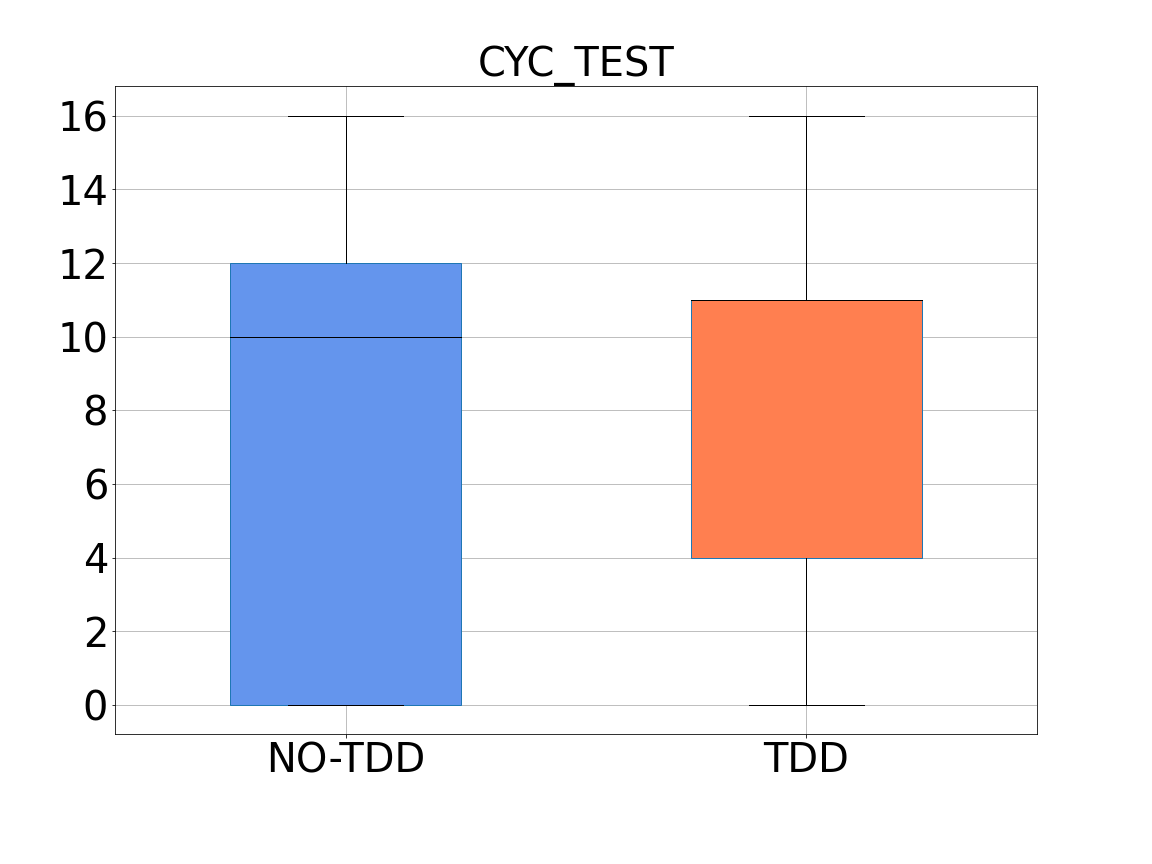
\includegraphics[width=\linewidth]{figures/box_plots/CYC_TEST.png}
        \caption{Cyclomatic complexity }
        \label{bp_task1_2_cyc_test}
    \end{subfigure}\hfil
    \begin{subfigure}{0.5\textwidth}
        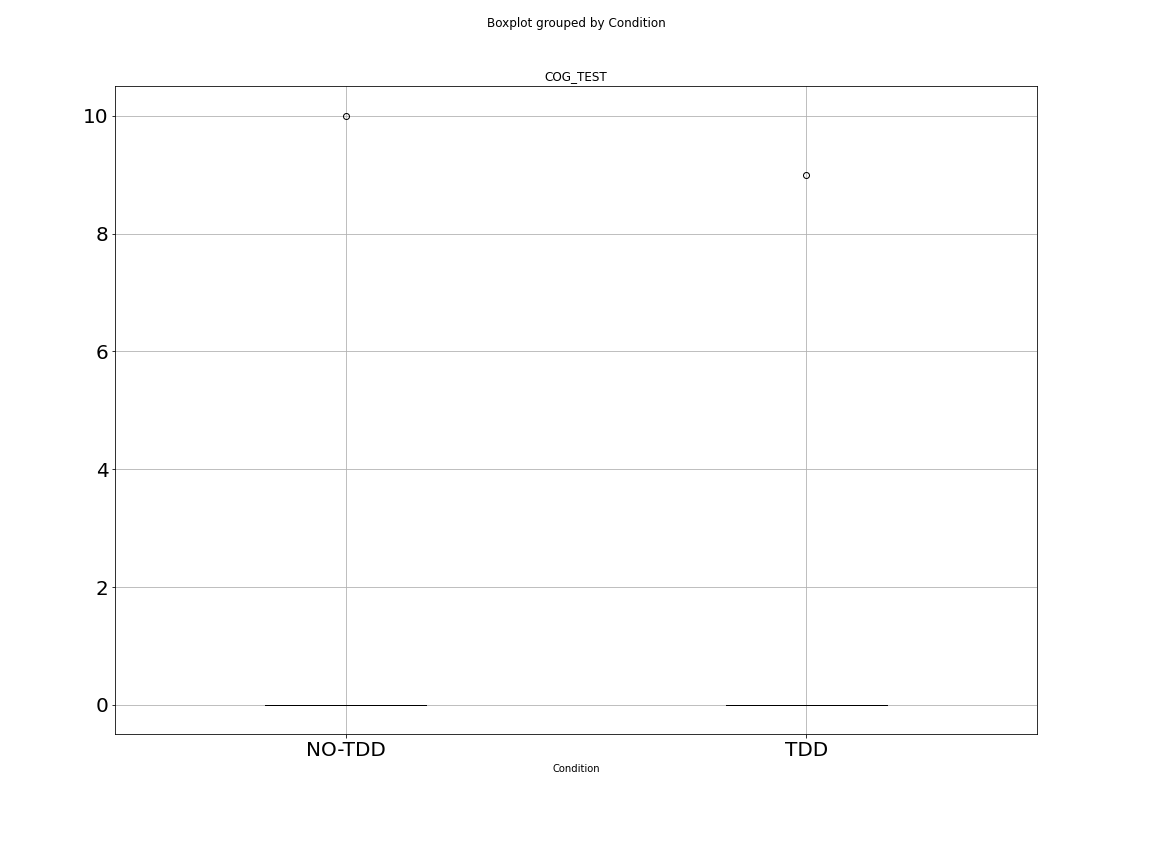
\includegraphics[width=\linewidth]{figures/box_plots/COG_TEST.png}
        \caption{Cognitive complexity}
        \label{bp_task1_2_cog_test}
    \end{subfigure}
    \caption{Box plots for the cyclomatic and cognitive complexities of test code for the first two tasks}
    \label{bp_task1_2_cyc_cog_test}
\end{figure}

Furthermore, we originally intended to also analyze the number of code smells in both the production and test code, however, as figure \ref{bp_task1_2_smells} highlights, there was no significant difference between the two approaches.

\begin{figure}[H]
    \centering
    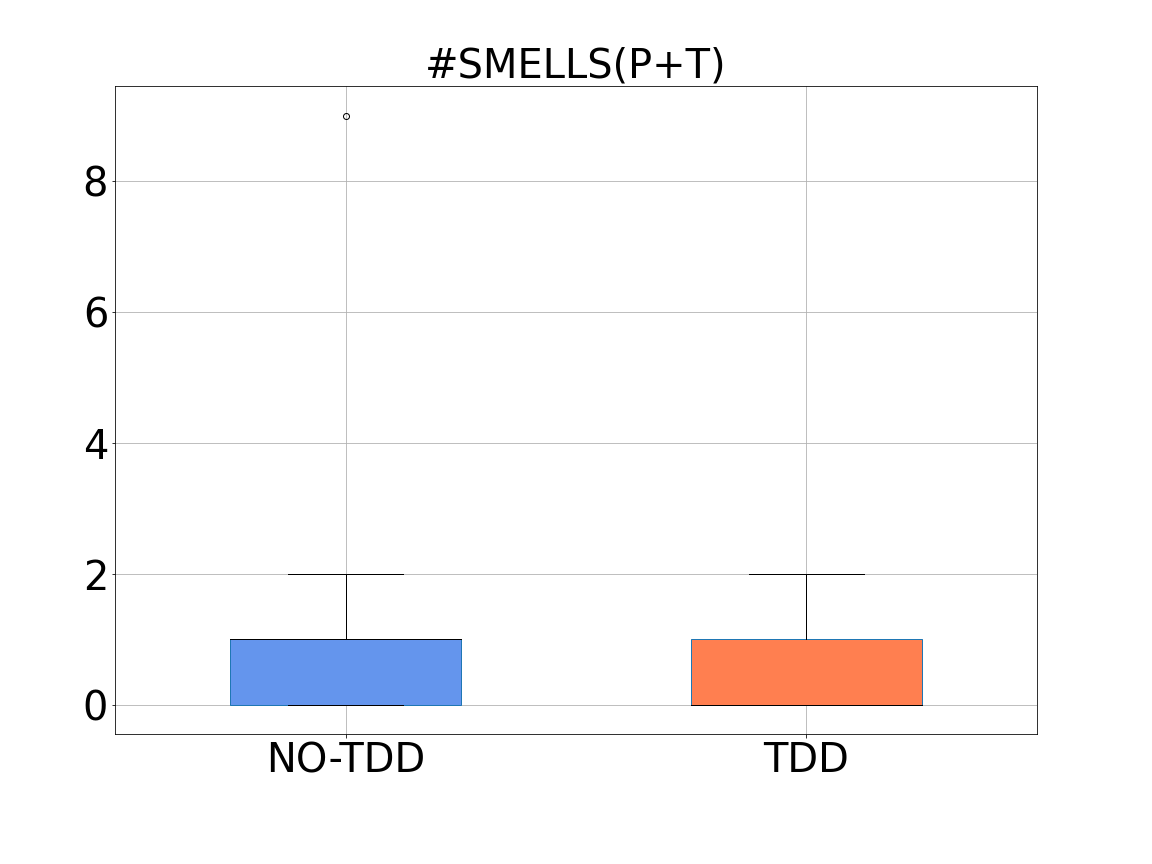
\includegraphics[width=0.5\linewidth, scale=0.5]{figures/box_plots/SMELLS.png}
    \caption{Number of code smells for the two tasks of \textit{Exp1}.}
    \label{bp_task1_2_smells}
\end{figure}


Starting with the first experimental task of \textit{Exp1}, table \ref{tab_dv_t1}, as well as figure \ref{box_plots_task1} show the tables containing the extracted statistical measures and the box plot charts for the dependent variables, respectively.

\begin{table}[H]
    \begin{center} 
        \begin{tabular}{|p{1.8cm}||p{1.6cm}|p{1.6cm}|p{1.6cm}|p{1.6cm}|p{1.6cm}|p{1.6cm}|}
            \hline
                \multicolumn{6}{|c|}{\textit{Exp1} - \textit{IO} - TDD} \\
            \hline
                Metric & Min & Max & Mean & Median & Std \\
            \hline
                QLTY & 73 & 96 & 81.12 & 77.77 & 10.73 \\
                PROD & 72 & 96 & 83 & 82 & 10 \\
                TEST & 8 & 10 & 9.5 & 10 & 1 \\
                CYC & 21 & 28 & 24.75 & 25 & 2.87 \\
                COG & 14 & 25 & 19 & 18.5 & 4.69 \\
                LOC & 154 & 195 & 167 & 159.5 & 18.95 \\
            \hline\hline
                \multicolumn{6}{|c|}{\textit{Exp1} - \textit{IO} - NO-TDD} \\
            \hline
                Metric & Min & Max & Mean & Median & Std\\
            \hline
                QLTY & 65.55 & 82 & 75.35 & 78.77 & 7.43 \\
                PROD & 56 & 84 & 76 & 80 & 11.66 \\
                TEST & 0 & 12 & 3.8 & 0 & 5.49 \\
                CYC & 12 & 18 & 15.6 & 16 & 2.19 \\
                COG & 9 & 17 & 14 & 15 & 3 \\
                LOC & 74 & 157 & 111.6 & 100 & 33.69 \\
            \hline
        \end{tabular}
        \caption{\label{tab_dv_t1}Dependent variables' statistics for task 1 of \textit{Exp1} - \textit{IO}}
    \end{center}
\end{table}

Here, $QLTY$ and $PROD$ paint the same picture, with both having a similar median and distribution of values among the two groups, with the group employing \tdd reporting slightly higher average and maximum values.
As for the number of written tests, every participant in \textit{G1} (\tdd), except for an outlier, wrote a similar number of tests (\ie 9 or 10), with a standard deviation of only 1, compared to \textit{G2}, where the number of written test cases fluctuates a lot more; still, however, the median for \textit{G2} is 0, since a few participants did not write any tests at all. Interestingly, the maximum value for $TEST$ in the \notdd group is higher than the maximum value for \tdd.
The other code quality metrics, $CYC$, $COG$, and $LOC$ are on average higher for the \tdd implementations, but still not significant (keep in mind that each function has a minimum cyclomatic complexity of 1, and the values here are considering the entire program).
A higher value of $LOC$ is generally expected for the \tdd implementation since this metric aggregates the lines of code in both the production code and the test files; however, even by considering the individual values for $LOC$ in the production and test files (not reported here), there is still not a significant difference in lines of code with respect to the implemented user stories, for both groups. We will however keep displaying the value of $LOC$ as an aggregated measurement, in order to highlight how the number of test cases impacts it.

\begin{figure}[H]
    \centering
    \begin{subfigure}{0.33\textwidth}
        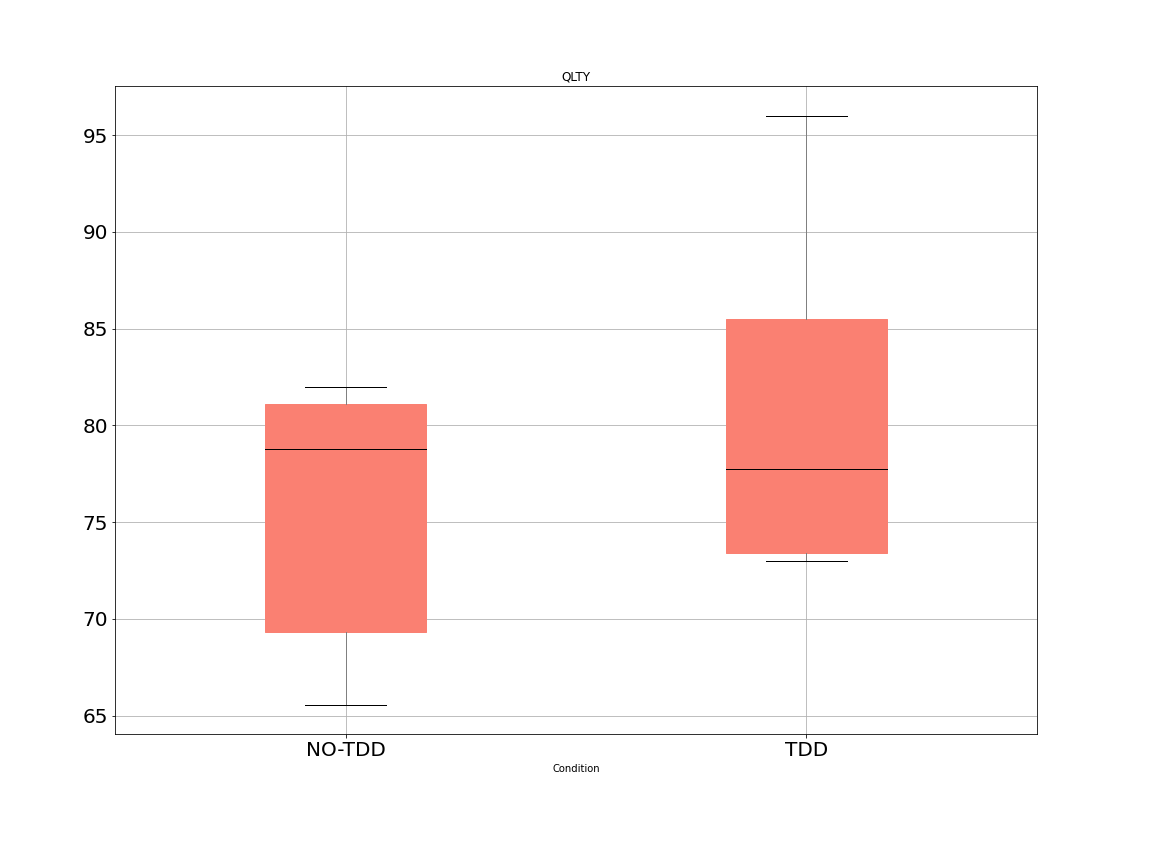
\includegraphics[width=\linewidth]{figures/box_plots/task1/QLTY.png}
        \caption{QLTY}
        \label{bp_task1_qlty}
    \end{subfigure}\hfil
        \begin{subfigure}{0.33\textwidth}
        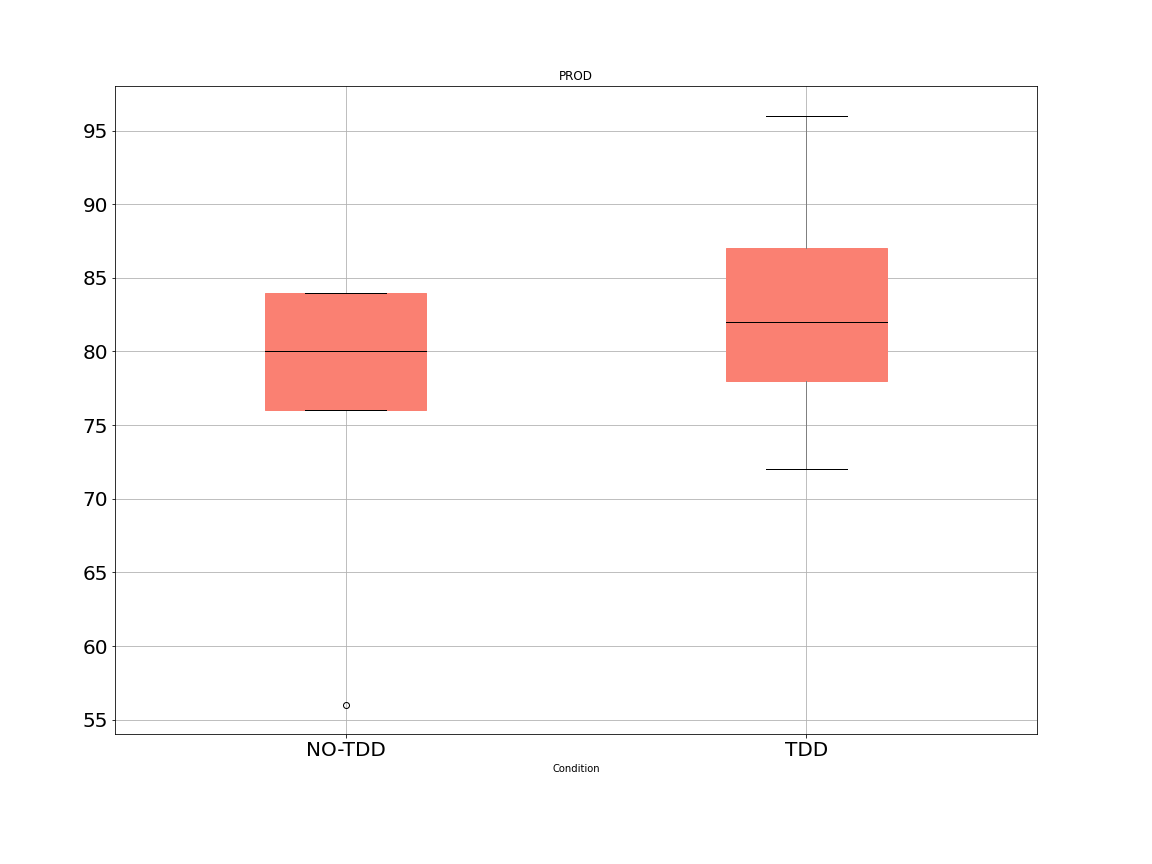
\includegraphics[width=\linewidth]{figures/box_plots/task1/PROD.png}
        \caption{PROD}
        \label{bp_task1_prod}
    \end{subfigure}\hfil
    \begin{subfigure}{0.33\textwidth}
        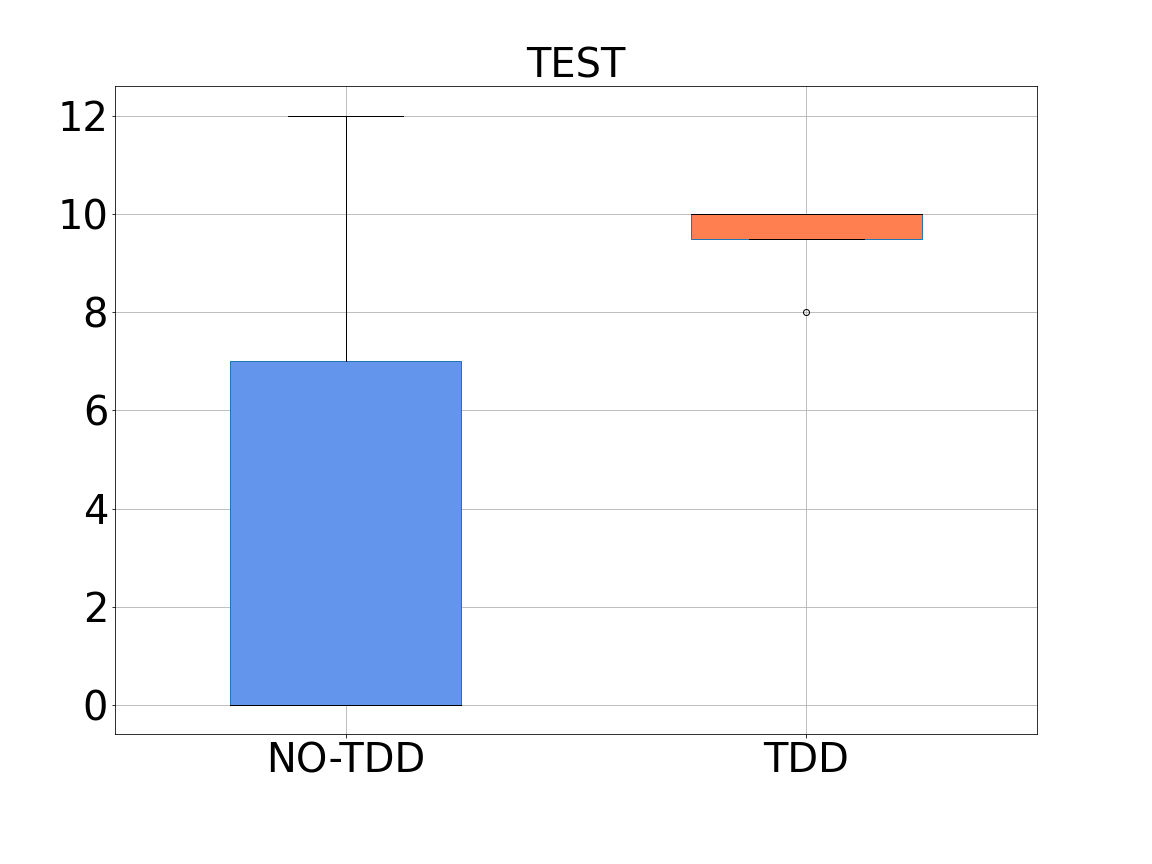
\includegraphics[width=\linewidth]{figures/box_plots/task1/TEST.png}
        \caption{TEST}
        \label{bp_task1_test}
    \end{subfigure}

    \medskip
    \begin{subfigure}{0.33\textwidth}
        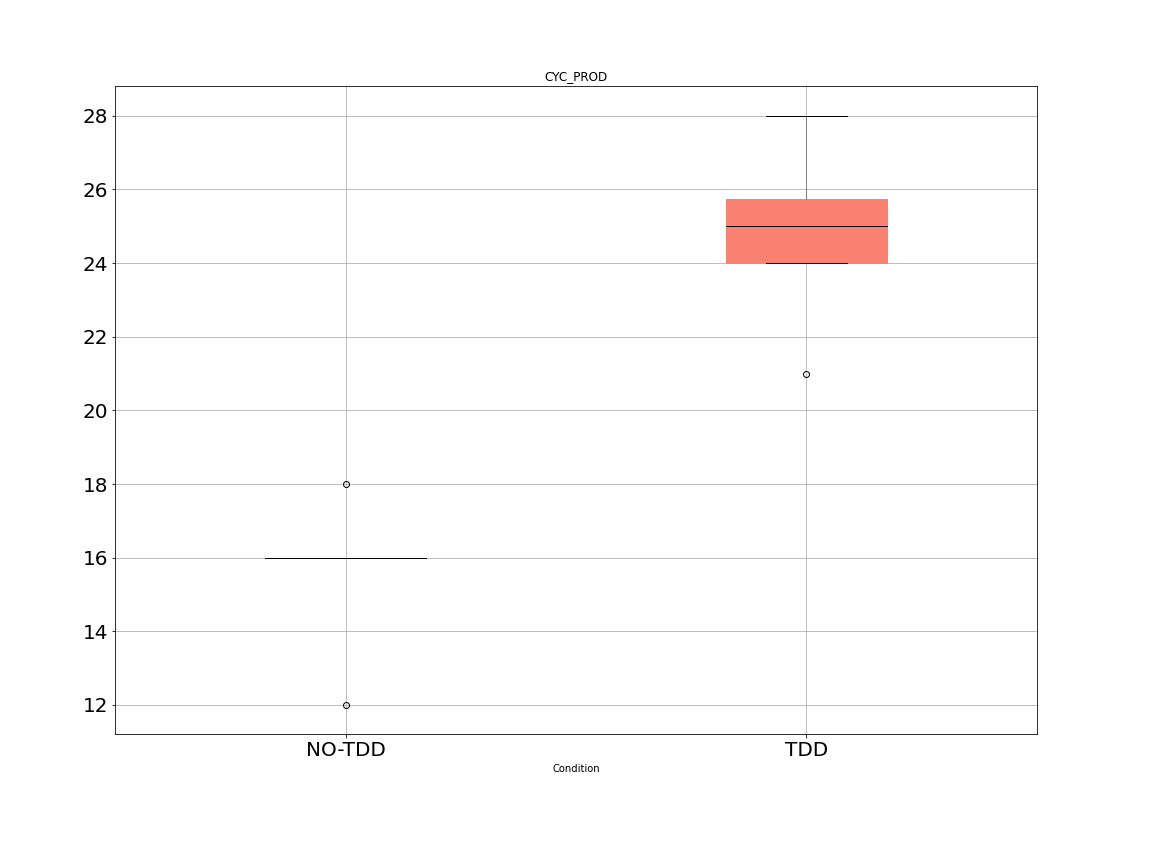
\includegraphics[width=\linewidth]{figures/box_plots/task1/CYC.png}
        \caption{CYC}
        \label{bp_task1_cyc}
    \end{subfigure}\hfil
    \begin{subfigure}{0.33\textwidth}
        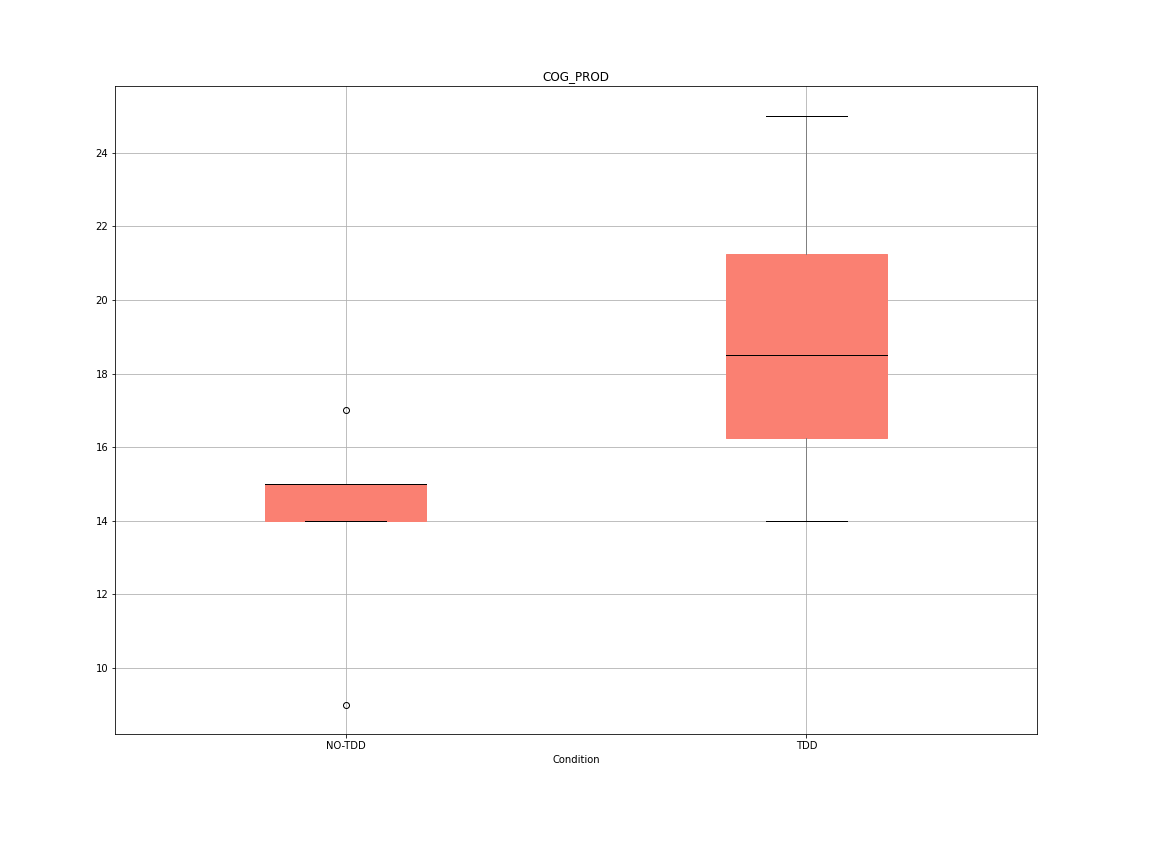
\includegraphics[width=\linewidth]{figures/box_plots/task1/COG.png}
        \caption{COG}
        \label{bp_task1_cog}
    \end{subfigure}\hfil
    \begin{subfigure}{0.33\textwidth}
        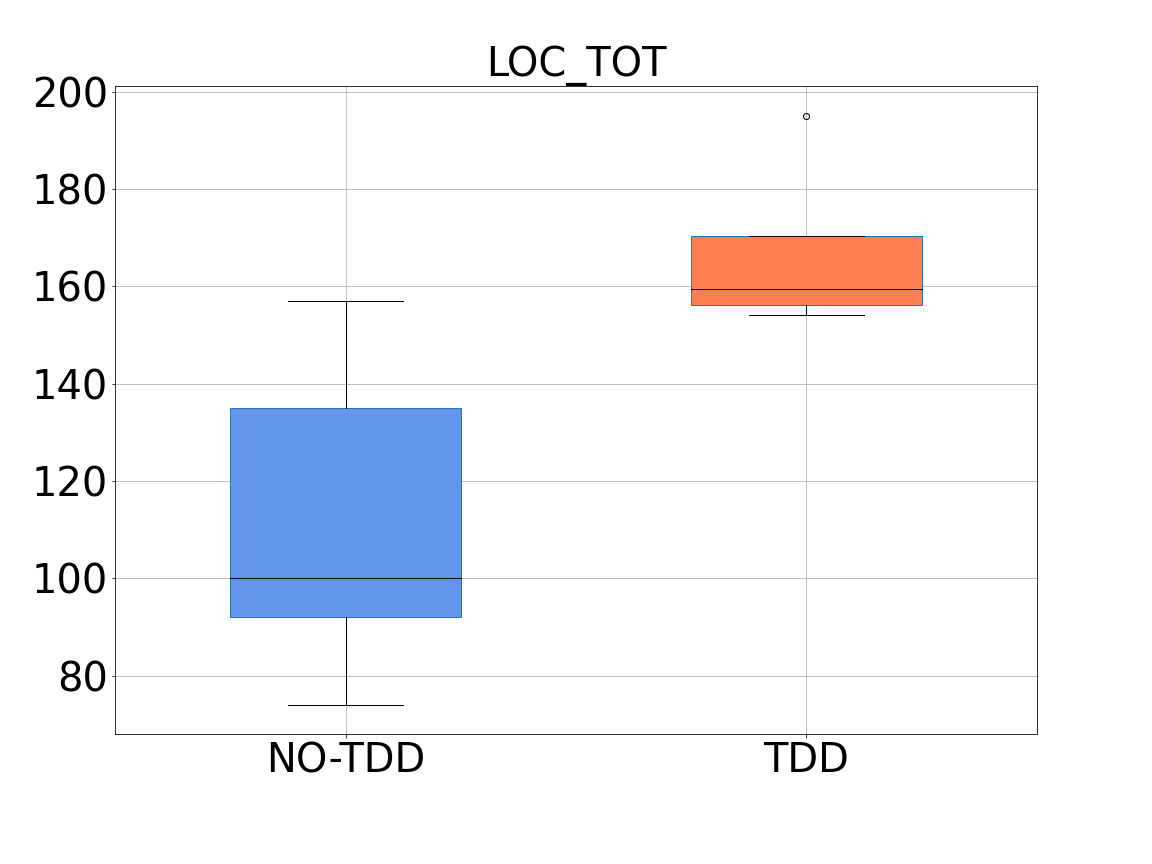
\includegraphics[width=\linewidth]{figures/box_plots/task1/LOC.png}
        \caption{LOC}
        \label{bp_task1_loc}
    \end{subfigure}
    \caption{Box plots for task 1 of \textit{Exp1} - \textit{IO}.}
    \label{box_plots_task1}
\end{figure}

In task 2 (which, as emerged from the post-questionnaires, many participants found harder compared to the previous one), the extracted statistics highlight the opposite situation (see table \ref{tab_dv_t2} and figure \ref{box_plots_task2}): while the values for $QLTY$ are still higher for the \tdd group (\textit{G2} in this case), the same thing is not true for $PROD$; this suggests that among the participants that tackled this task using \tdd, there are some that only tackled the first user stories, and did so flawlessly, thus resulting in a high value for $QLTY$ (100\% median, and 84\% mean), and a much lower value for $PROD$ (21\% median and 38.6\% mean). 
For the same reason, the average number of tests written is lower (5.4 average for \textit{G2} compared to the 9 average for \textit{G1}); the maximum value, however, is still higher for \textit{G2}, possibly resulting from a participant more extensively applying \tdd to all user stories of the task.
Finally, this time the values of $CYC$ and $COG$ are higher for the \notdd group; this is just related to the latter implementing overall more stories. The $LOC$ displays a similar behavior.


\begin{table}[H]
    \begin{center} 
        \begin{tabular}{ |p{2cm}||p{1.6cm}|p{1.6cm}|p{1.6cm}|p{1.6cm}|p{1.6cm}|}
            \hline
                \multicolumn{6}{|c|}{\textit{Exp1} - \textit{CR} - TDD} \\
            \hline
                Metric & Min & Max & Mean & Median & Std\\
            \hline
                QLTY & 50 & 100 & 84.44 & 100 & 22.70 \\
                PROD & 8 & 100 & 38.6 & 21 & 37.35 \\
                TEST & 0 & 13 & 5.4 & 3 & 5.12 \\
                CYC & 9 & 19 & 12 & 10 & 4.06 \\
                COG & 2 & 40 & 12.8 & 4.0 & 15.91 \\
                LOC & 80 & 203 & 128 & 115 & 45.61 \\
            \hline\hline
                \multicolumn{6}{|c|}{\textit{Exp1} - \textit{CR} - NO-TDD} \\
            \hline
                Metric & Min & Max & Mean & Median & Std\\
            \hline
                QLTY & 74 & 94.43 & 83.07 & 81.94 & 10.17 \\
                PROD & 52 & 73 & 60.5 & 58.5 & 10.24 \\
                TEST & 5 & 12 & 9 & 9.5 & 2.94 \\
                CYC & 16 & 36 & 23.5 & 21 & 9 \\
                COG & 11 & 49 & 29 & 28 & 15.57 \\
                LOC & 178 & 260 & 207.5 & 196 & 37.11 \\
            \hline
        \end{tabular}
        \caption{\label{tab_dv_t2}Dependent variables' statistics for task 2 of \textit{Exp1} - \textit{CR}.}
    \end{center}
\end{table}

In the task developed for \textit{Exp2}, on the other hand, (see table \ref{tab_dv_t3} and figure \ref{box_plots_task3}), we see something much more in line with the first experimental task, with results in favor of \tdd.
First, $QLTY$ and $PROD$ have a similar distribution of values for both approaches, suggesting that all stories that have been tackled are ``balanced" (\ie there is no hard user story like there was in task 2); the \tdd group produced results that are around 10\% better on average.
For the number of tests, we see again a result in line with the first task, with the \tdd group producing on average many more tests, and with the minimum value for this group still well above the median of 3.5 for the \notdd group.
Regarding the three last variables associated with code complexity and quality, once again these are higher for the \tdd approach, even though, in the case of cyclomatic and cognitive complexity, the result are still not concerning from a maintainability point of view.

\begin{figure}[H]
    \centering
    \begin{subfigure}{0.33\textwidth}
        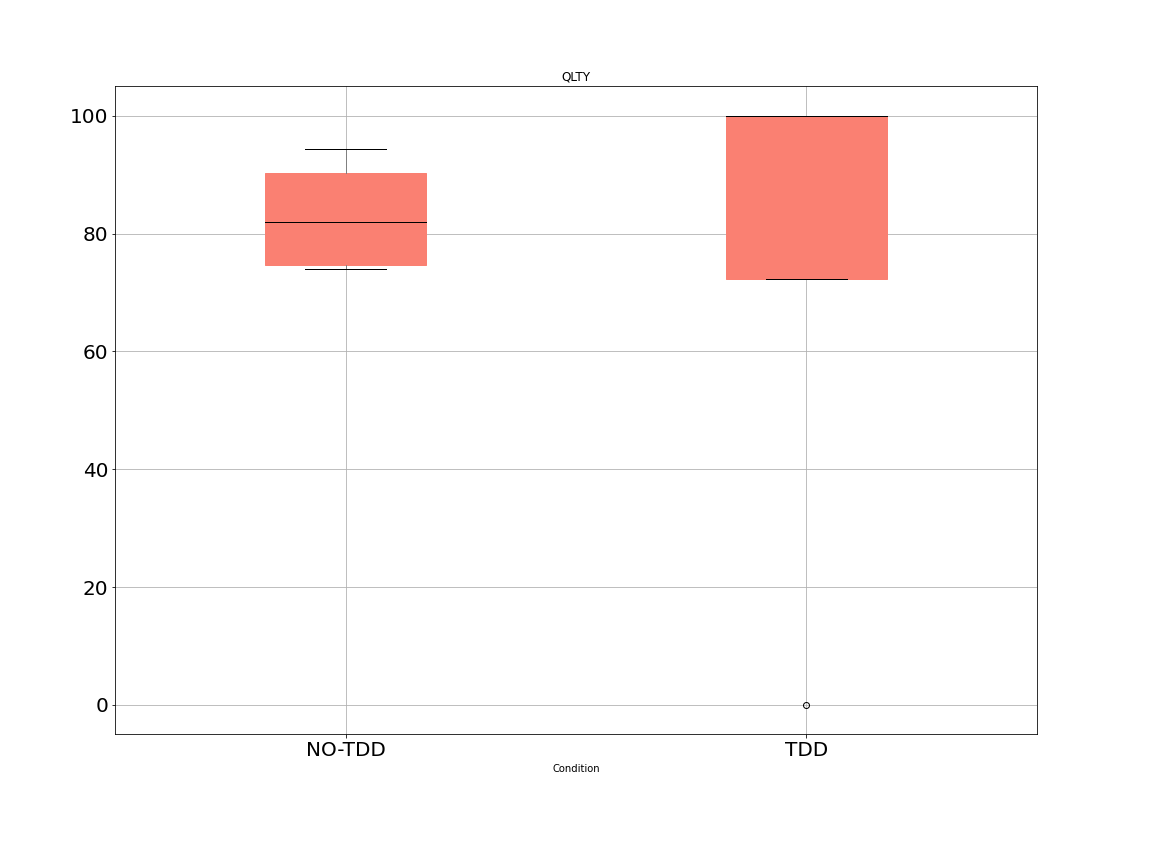
\includegraphics[width=\linewidth]{figures/box_plots/task2/QLTY.png}
        \caption{QLTY}
        \label{bp_task2_qlty}
    \end{subfigure}\hfil
        \begin{subfigure}{0.33\textwidth}
        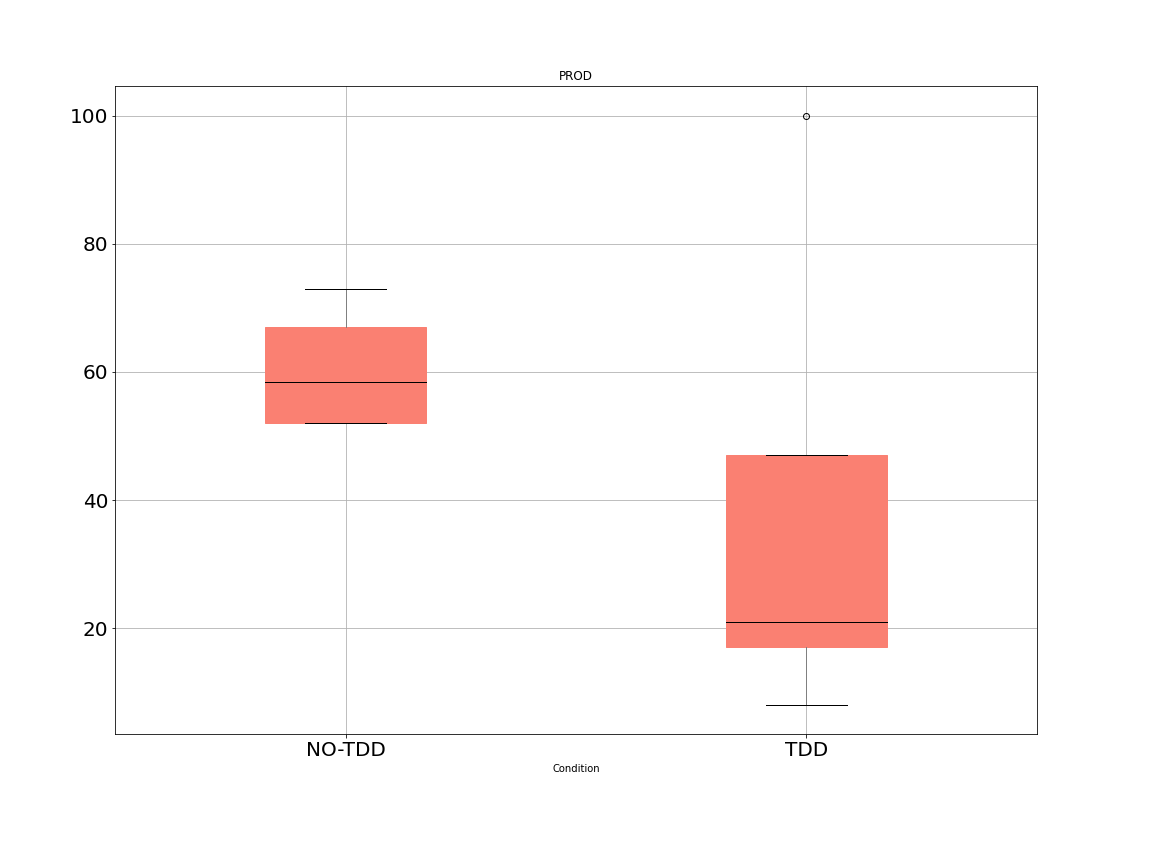
\includegraphics[width=\linewidth]{figures/box_plots/task2/PROD.png}
        \caption{PROD}
        \label{bp_task2_prod}
    \end{subfigure}\hfil
    \begin{subfigure}{0.33\textwidth}
        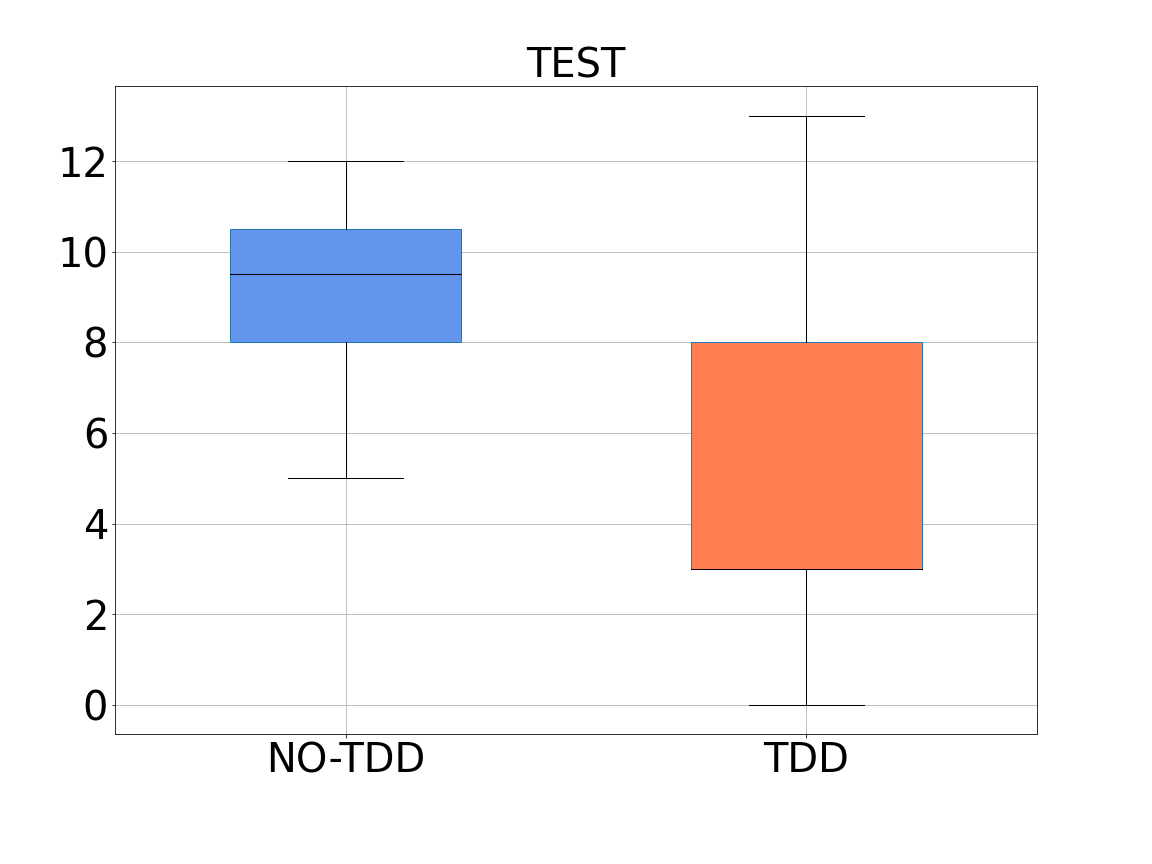
\includegraphics[width=\linewidth]{figures/box_plots/task2/TEST.png}
        \caption{TEST}
        \label{bp_task2_test}
    \end{subfigure}

    \medskip
    \begin{subfigure}{0.33\textwidth}
        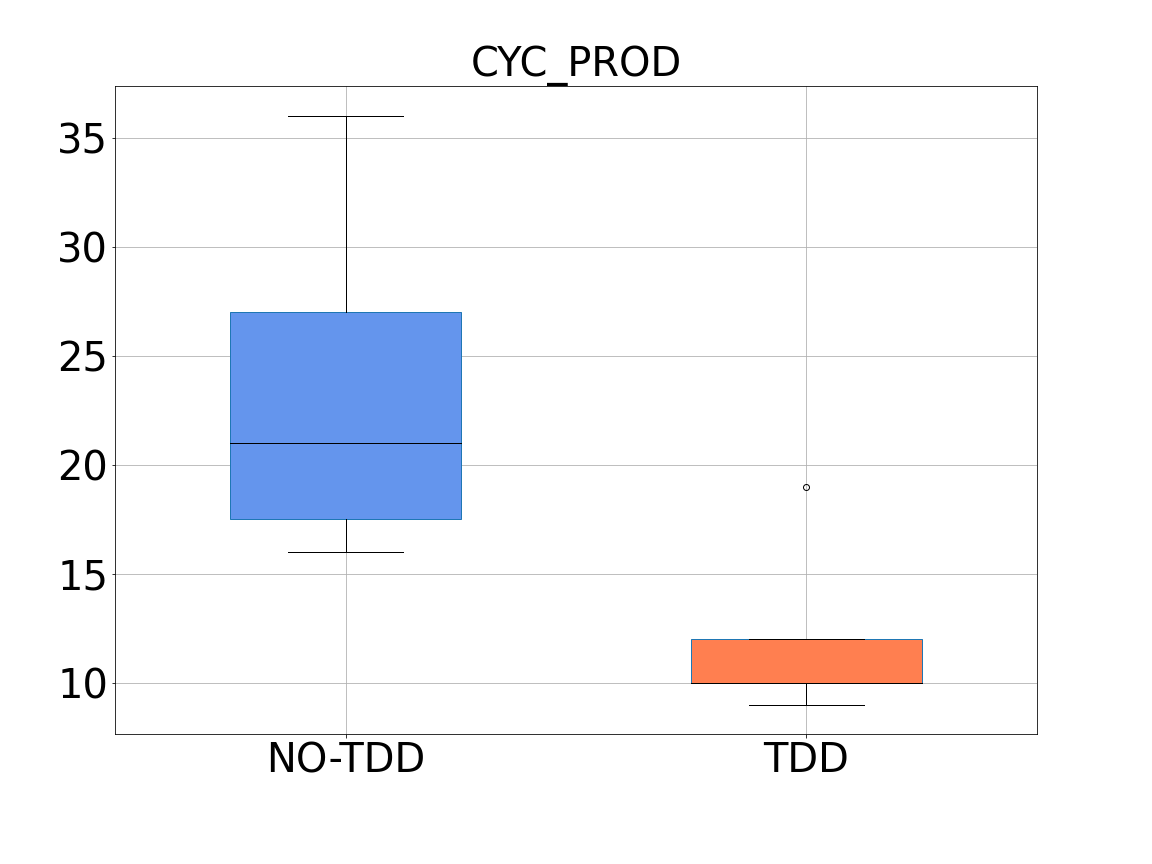
\includegraphics[width=\linewidth]{figures/box_plots/task2/CYC.png}
        \caption{CYC}
        \label{bp_task2_cyc}
    \end{subfigure}\hfil
    \begin{subfigure}{0.33\textwidth}
        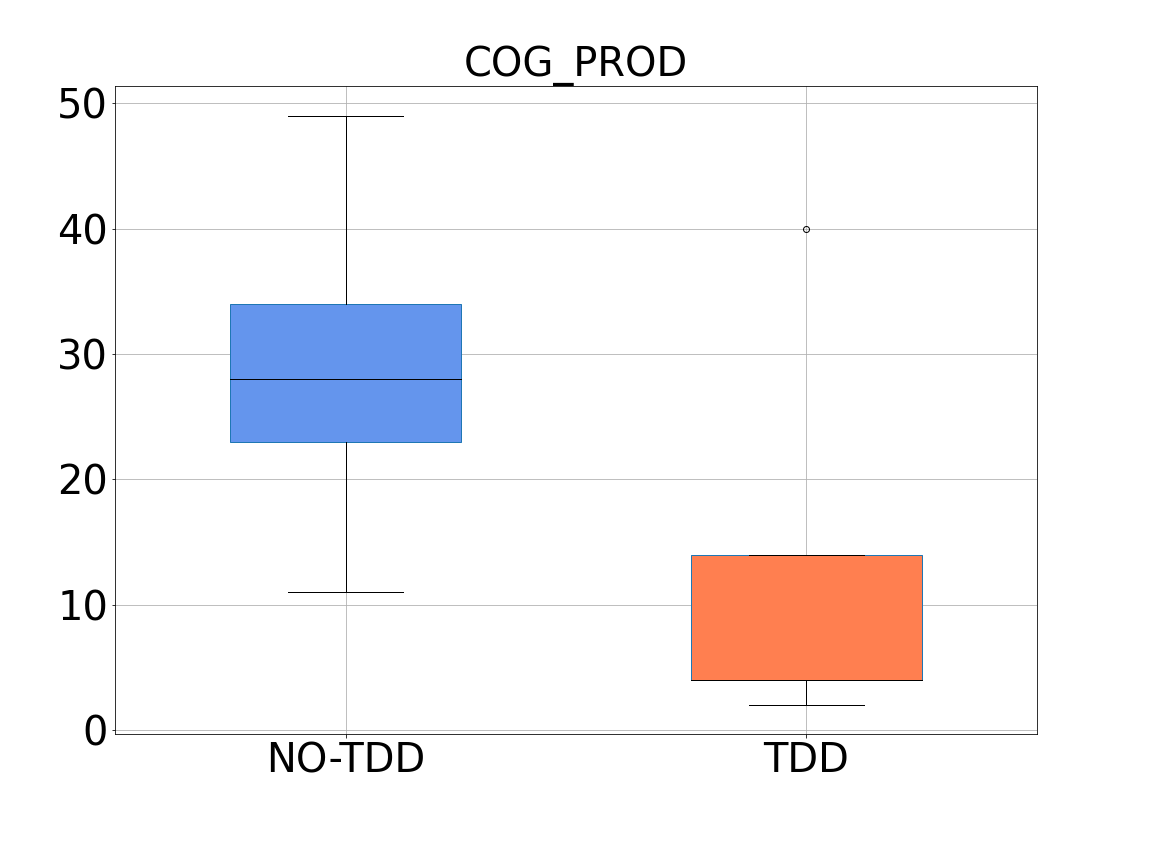
\includegraphics[width=\linewidth]{figures/box_plots/task2/COG.png}
        \caption{COG}
        \label{bp_task2_cog}
    \end{subfigure}\hfil
    \begin{subfigure}{0.33\textwidth}
        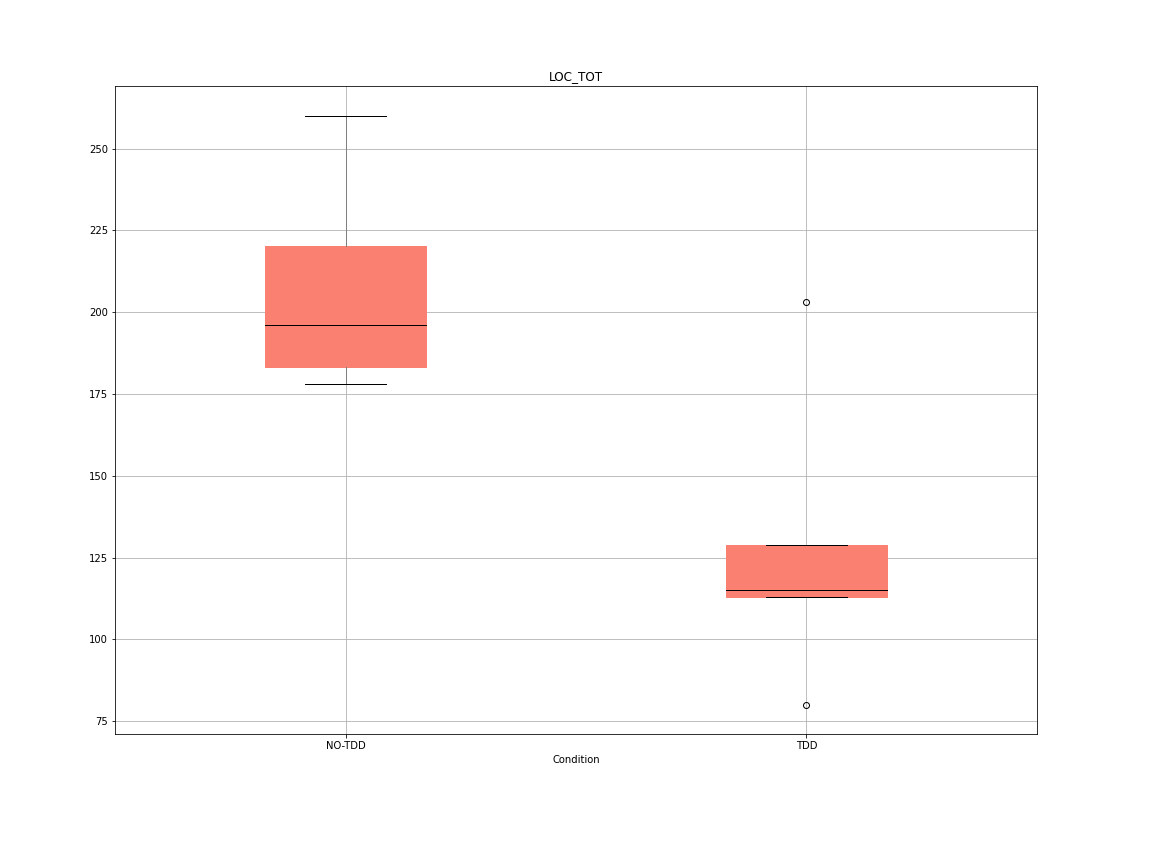
\includegraphics[width=\linewidth]{figures/box_plots/task2/LOC.png}
        \caption{LOC}
        \label{bp_task2_loc}
    \end{subfigure}
    \caption{Box plots for task 2 of \textit{Exp1} - \textit{CR}.}
    \label{box_plots_task2}
\end{figure}

\begin{table}[H]
    \begin{center} 
        \begin{tabular}{ |p{2cm}||p{1.6cm}|p{1.6cm}|p{1.6cm}|p{1.6cm}|p{1.6cm}|}
            \hline
                \multicolumn{6}{|c|}{\textit{Exp2} - TDD} \\
            \hline
                Metric & Min & Max & Mean & Median & Std\\
            \hline
                QLTY & 85 & 100 & 95 & 100 & 7.07 \\
                PROD & 83.33 & 100 & 93.33 & 100 & 9.13 \\
                TEST & 7 & 18 & 11.6 & 12 & 4.15 \\
                CYC & 15 & 30 & 22.6 & 20 & 6.58 \\
                COG & 18 & 34 & 25.8 & 25 & 7.08 \\
                LOC & 150 & 232 & 187 & 175 & 36.15 \\
            \hline\hline
                \multicolumn{6}{|c|}{\textit{Exp2} - NO-TDD} \\
            \hline
                Metric & Min & Max & Mean & Median & Std\\
            \hline
                QLTY & 80 & 100 & 86.25 & 82.5 & 9.46 \\
                PROD & 75 & 100 & 83.33 & 79.16 & 11.78 \\
                TEST & 0 & 11 & 4.5 & 3.5 & 5.44 \\
                CYC & 16 & 23 & 19.5 & 19.5 & 2.88 \\
                COG & 19 & 25 & 21 & 20 & 2.70 \\
                LOC & 93 & 164 & 125.5 & 122.5 & 36.82 \\
            \hline
        \end{tabular}
        \caption{\label{tab_dv_t3}Dependent variables' statistics for \textit{Exp2}.}
    \end{center}
\end{table}

\begin{figure}[H]
    \centering
    \begin{subfigure}{0.33\textwidth}
        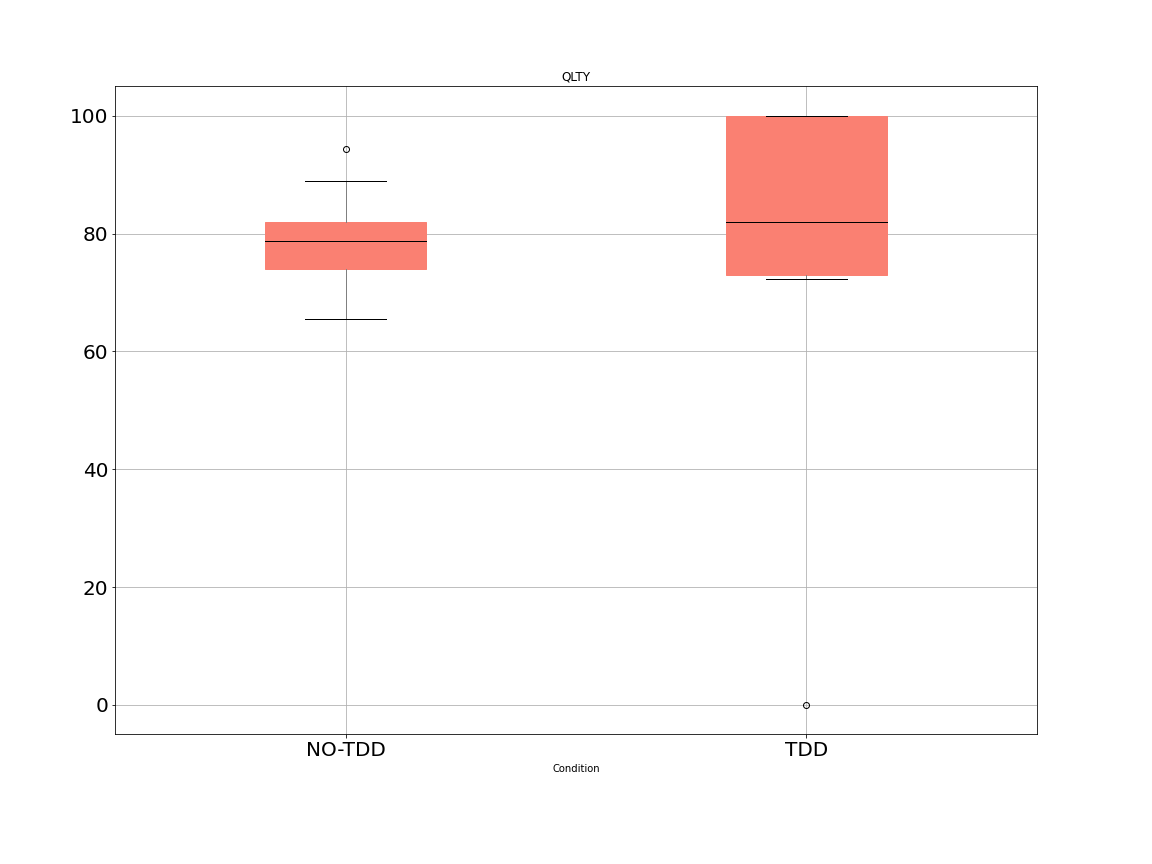
\includegraphics[width=\linewidth]{figures/box_plots/task1_2/QLTY.png}
        \caption{QLTY}
        \label{bp_task1_2_qlty}
    \end{subfigure}\hfil
        \begin{subfigure}{0.33\textwidth}
        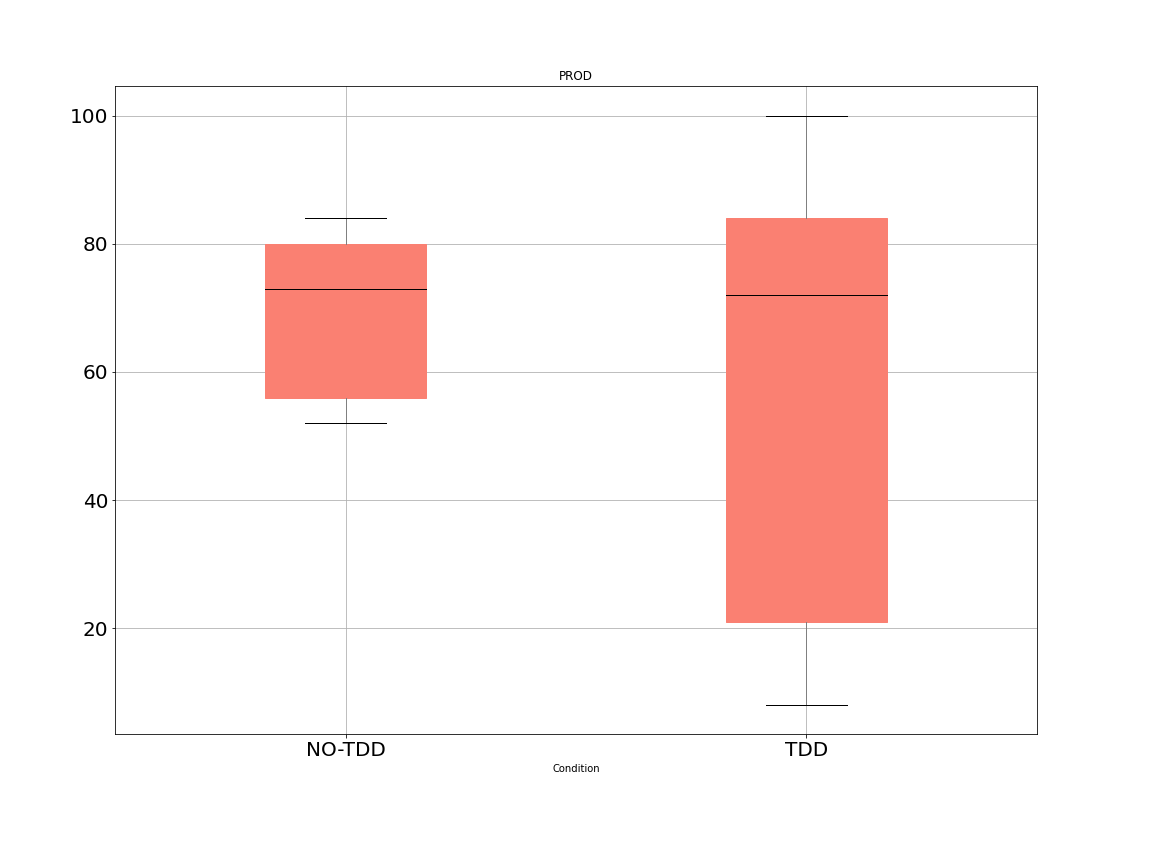
\includegraphics[width=\linewidth]{figures/box_plots/task1_2/PROD.png}
        \caption{PROD}
        \label{bp_task1_2_prod}
    \end{subfigure}\hfil
    \begin{subfigure}{0.33\textwidth}
        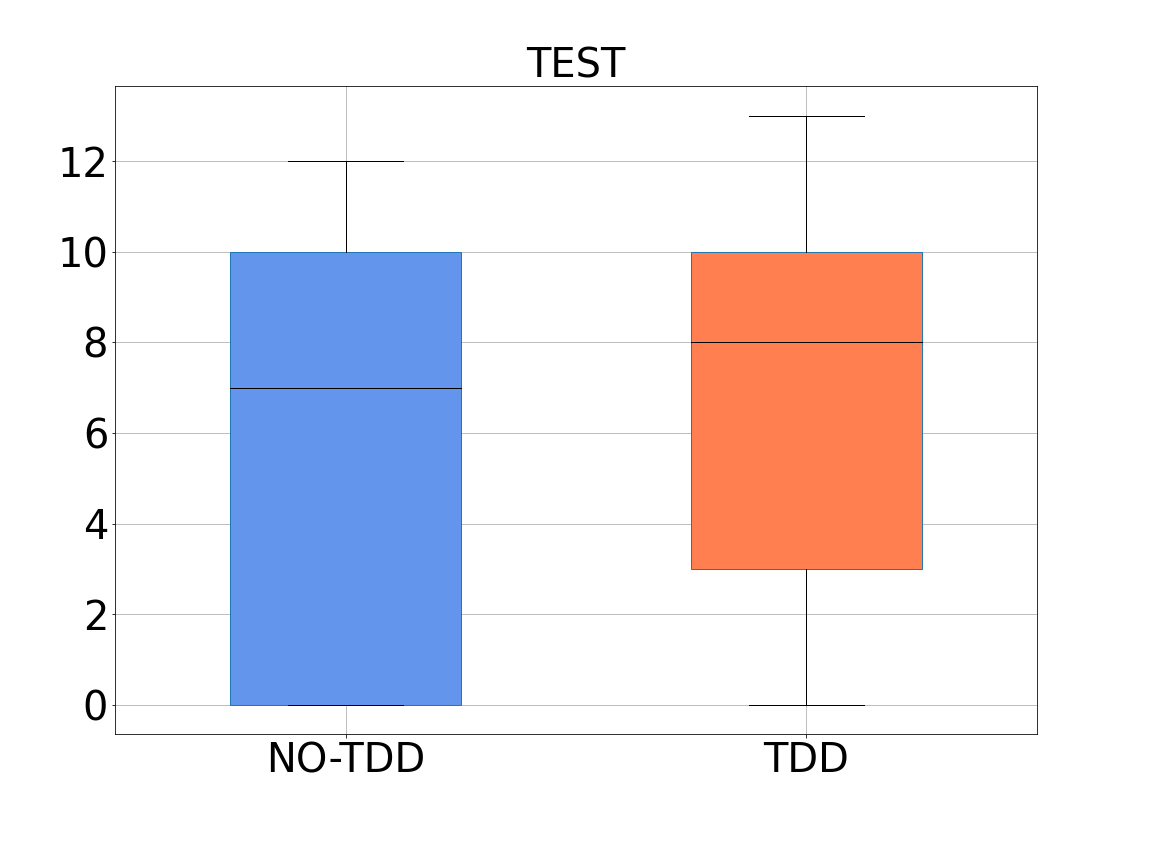
\includegraphics[width=\linewidth]{figures/box_plots/task1_2/TEST.png}
        \caption{TEST}
        \label{bp_task1_2_test}
    \end{subfigure}

    \medskip
    \begin{subfigure}{0.33\textwidth}
        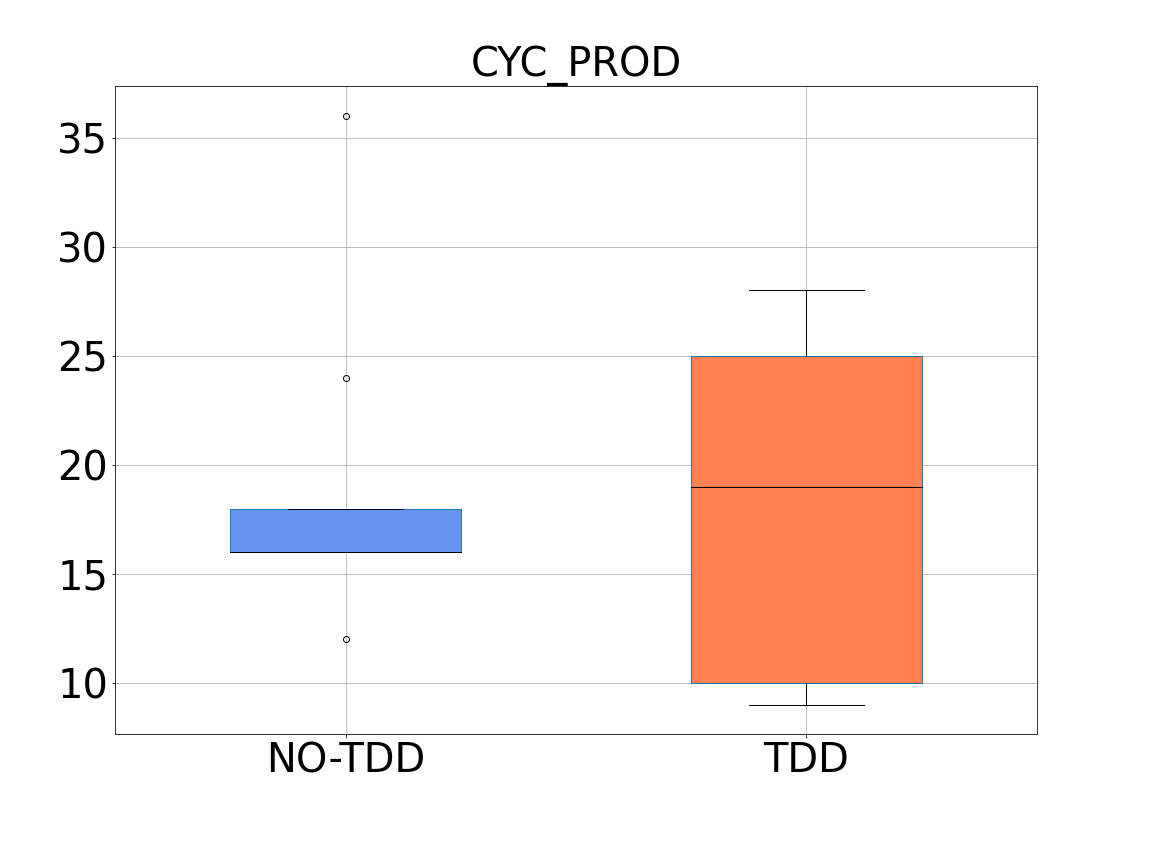
\includegraphics[width=\linewidth]{figures/box_plots/task1_2/CYC.png}
        \caption{CYC}
        \label{bp_task1_2_cyc}
    \end{subfigure}\hfil
    \begin{subfigure}{0.33\textwidth}
        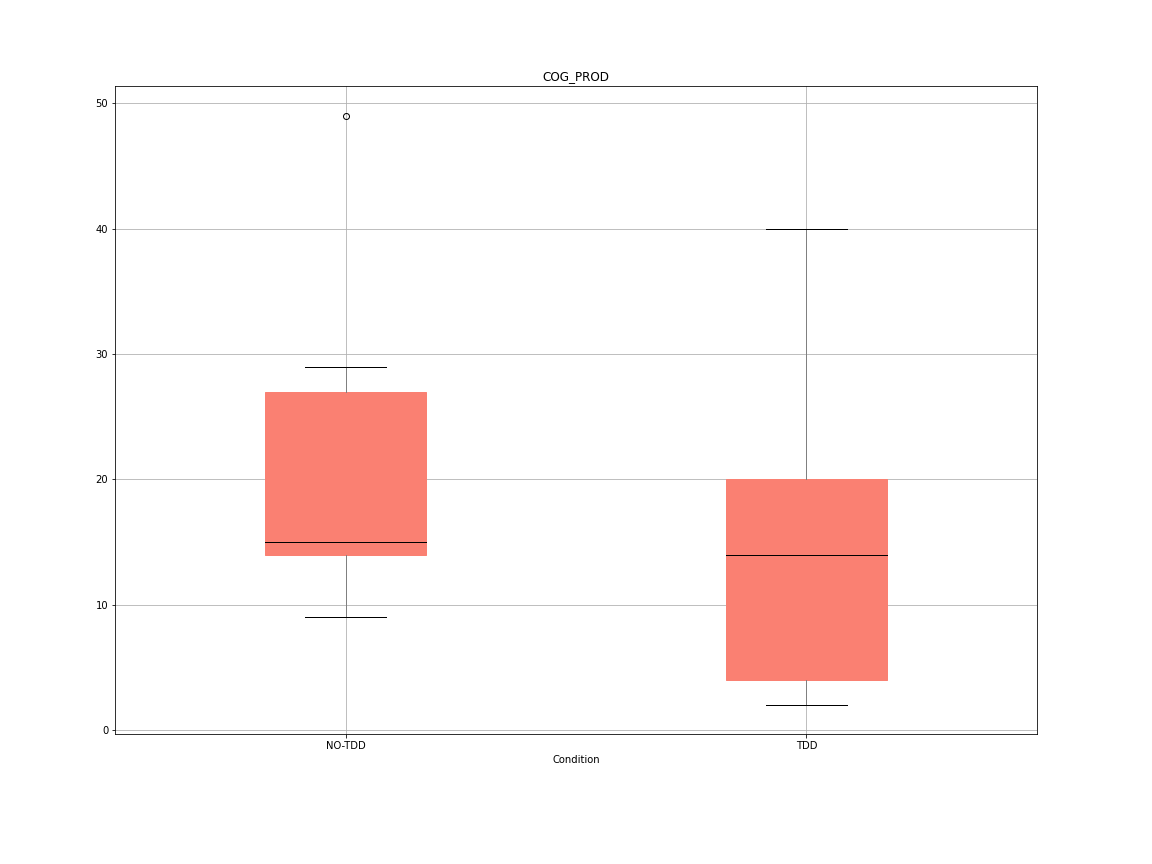
\includegraphics[width=\linewidth]{figures/box_plots/task1_2/COG.png}
        \caption{COG}
        \label{bp_task1_2_cog}
    \end{subfigure}\hfil
    \begin{subfigure}{0.33\textwidth}
        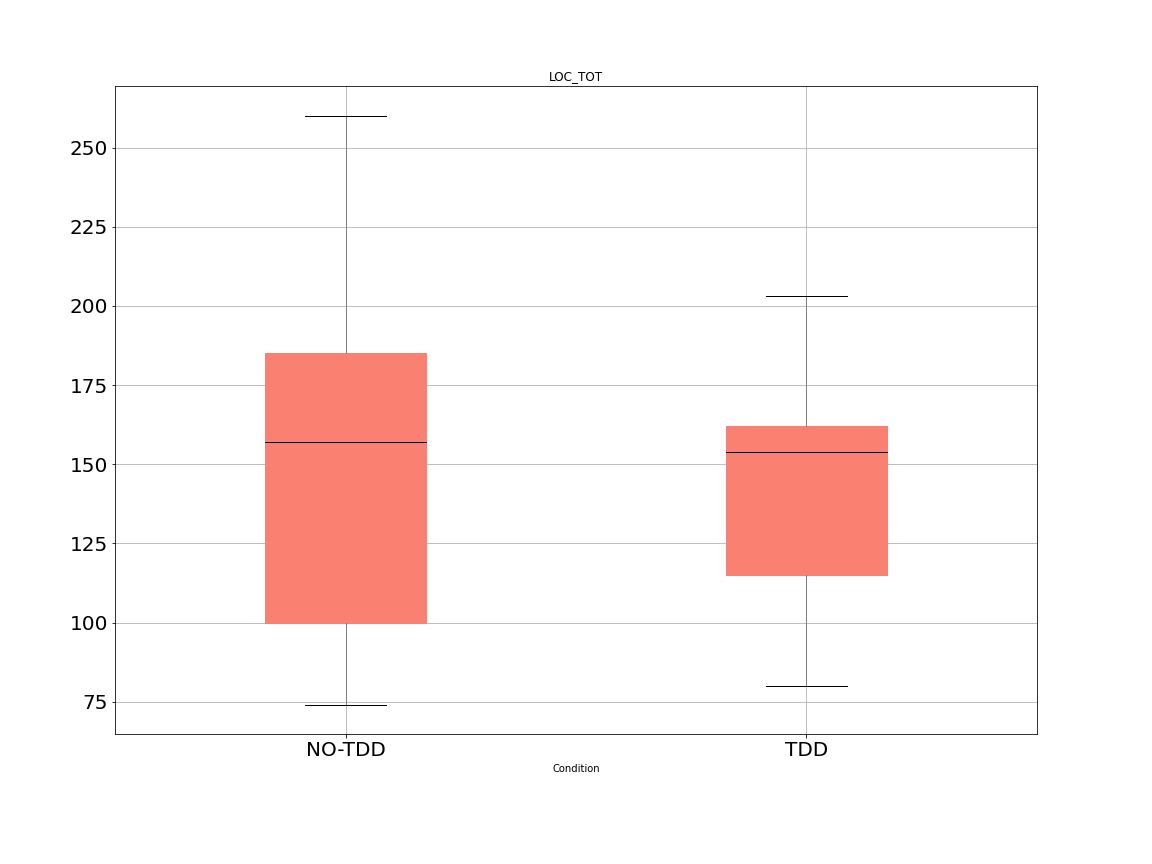
\includegraphics[width=\linewidth]{figures/box_plots/task1_2/LOC.png}
        \caption{LOC}
        \label{bp_task1_2_loc}
    \end{subfigure}
    \caption{Aggregated box plot charts for \textit{Exp1}.}
    \label{box_plots_task1_2}
\end{figure}


\begin{figure}[htbp]
    \centering
    \begin{subfigure}{0.33\textwidth}
        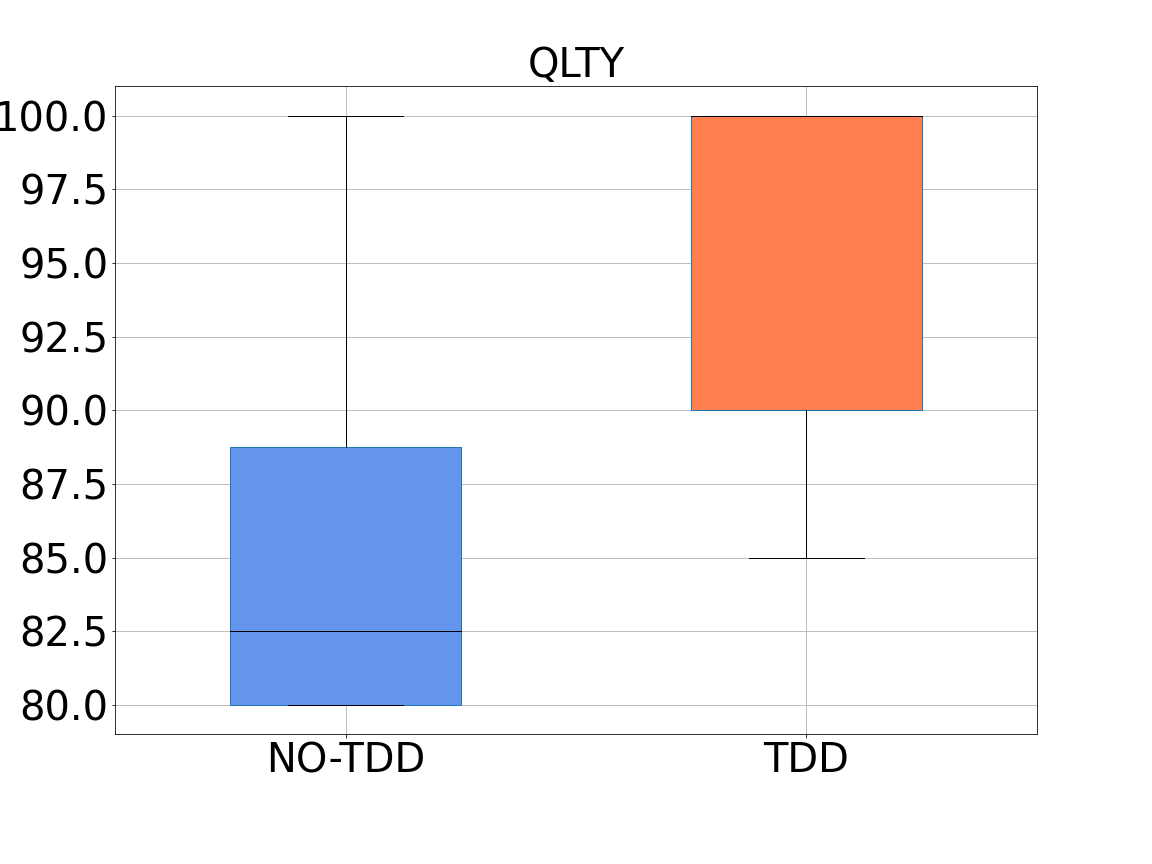
\includegraphics[width=\linewidth]{figures/box_plots/task3/QLTY.png}
        \caption{QLTY}
        \label{bp_task3_qlty}
    \end{subfigure}\hfil
        \begin{subfigure}{0.33\textwidth}
        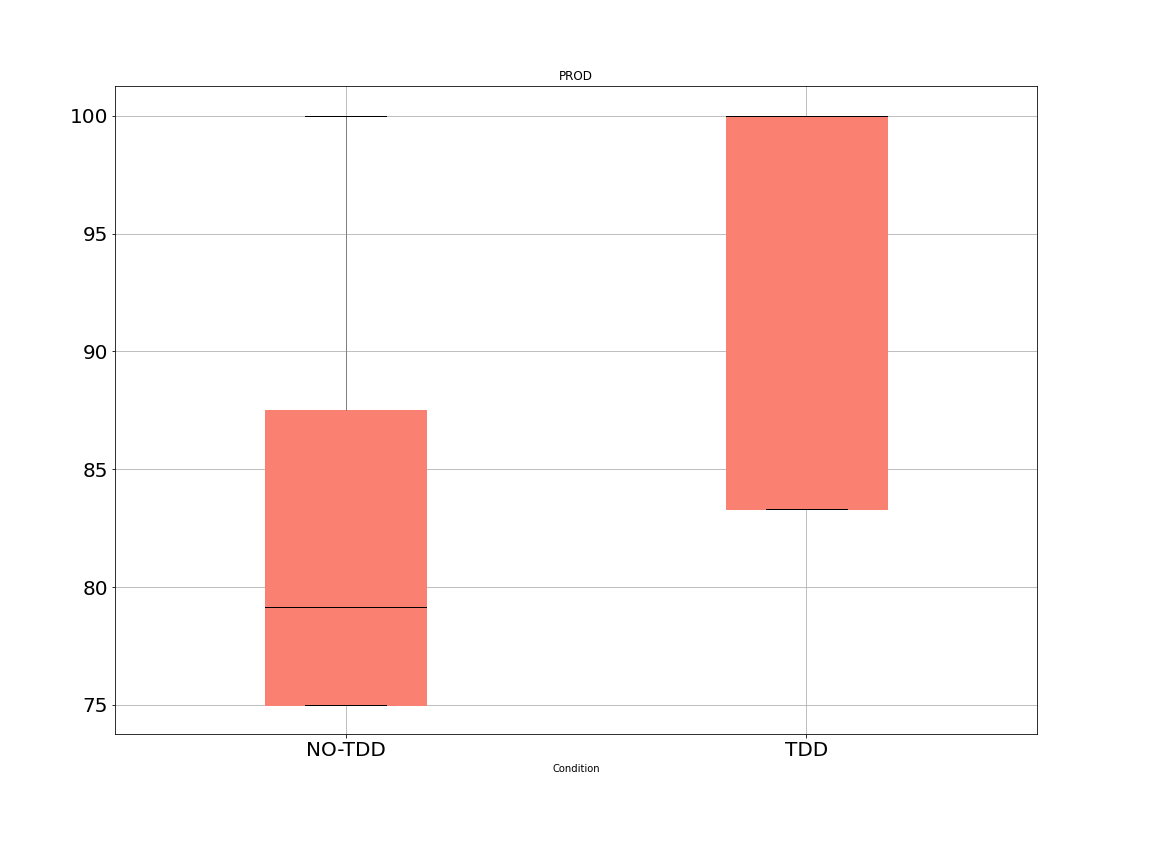
\includegraphics[width=\linewidth]{figures/box_plots/task3/PROD.png}
        \caption{PROD}
        \label{bp_task3_prod}
    \end{subfigure}\hfil
    \begin{subfigure}{0.33\textwidth}
        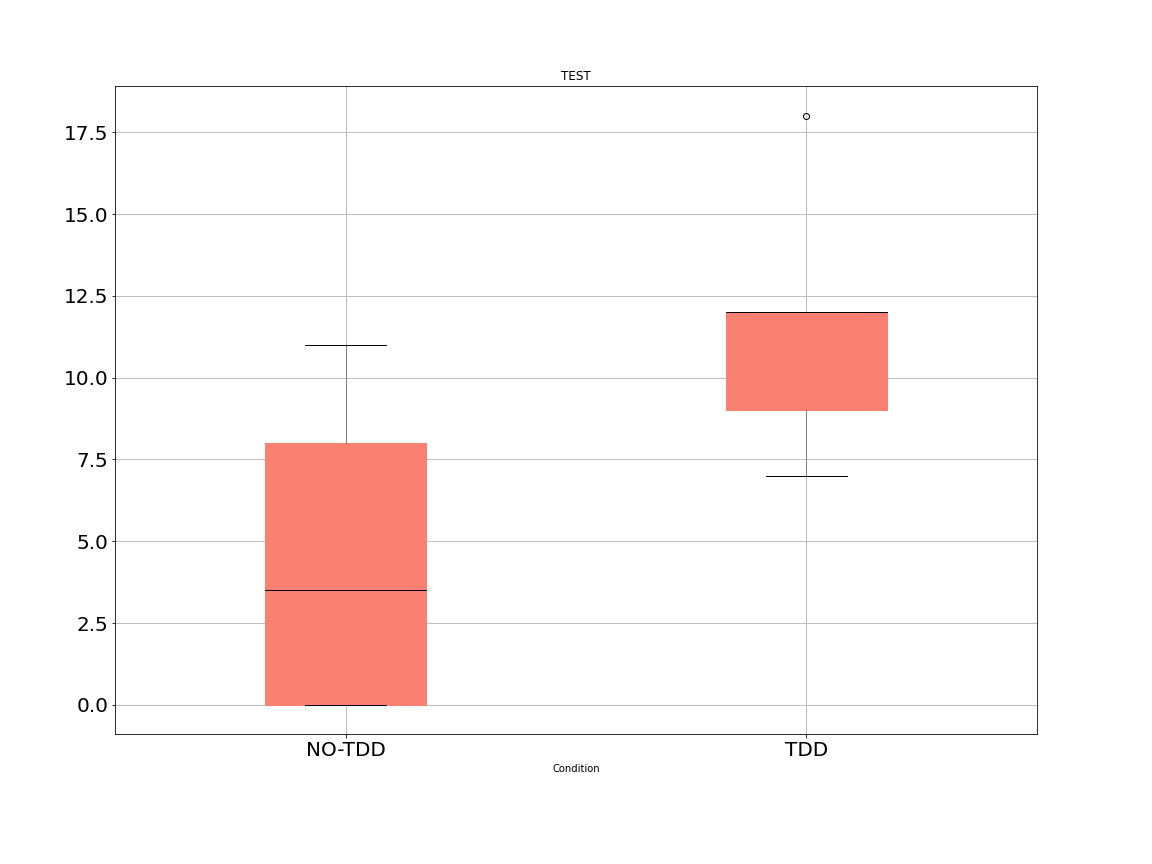
\includegraphics[width=\linewidth]{figures/box_plots/task3/TEST.png}
        \caption{TEST}
        \label{bp_task3_test}
    \end{subfigure}

    \medskip
    \begin{subfigure}{0.33\textwidth}
        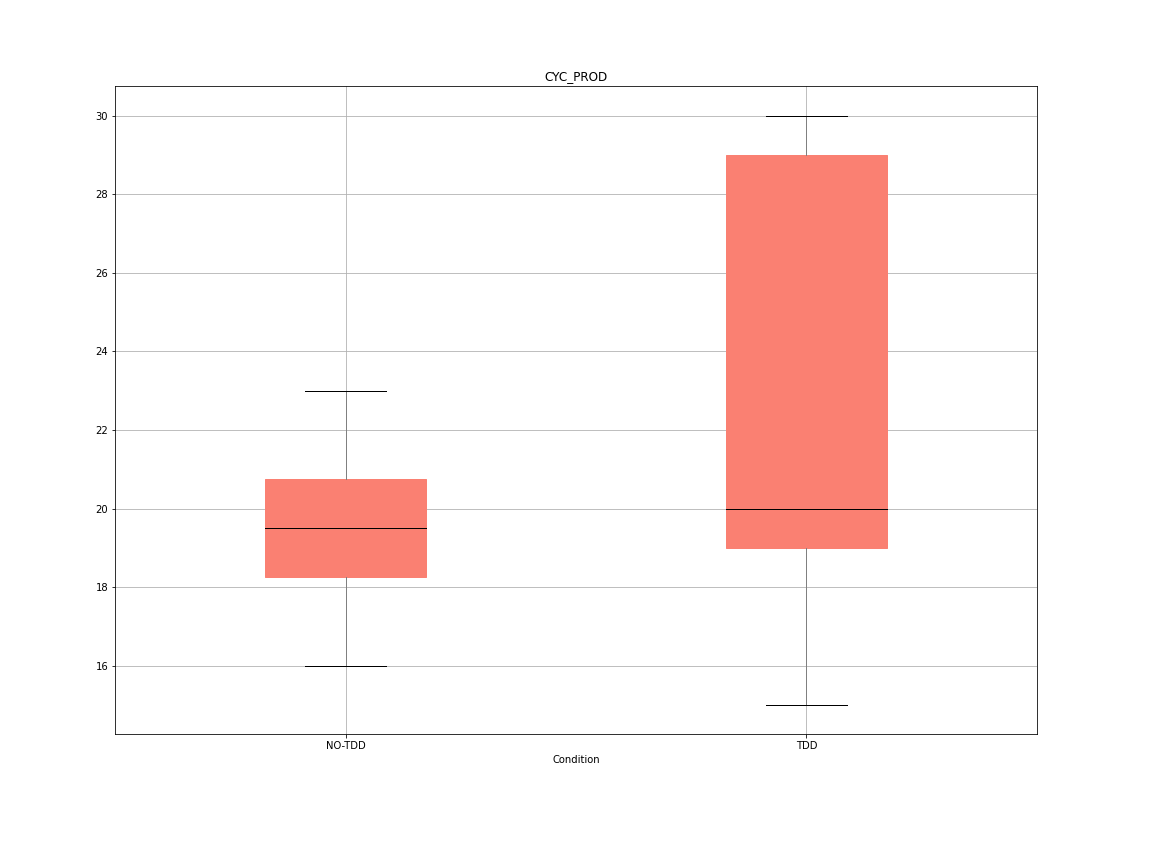
\includegraphics[width=\linewidth]{figures/box_plots/task3/CYC.png}
        \caption{CYC}
        \label{bp_task3_cyc}
    \end{subfigure}\hfil
    \begin{subfigure}{0.33\textwidth}
        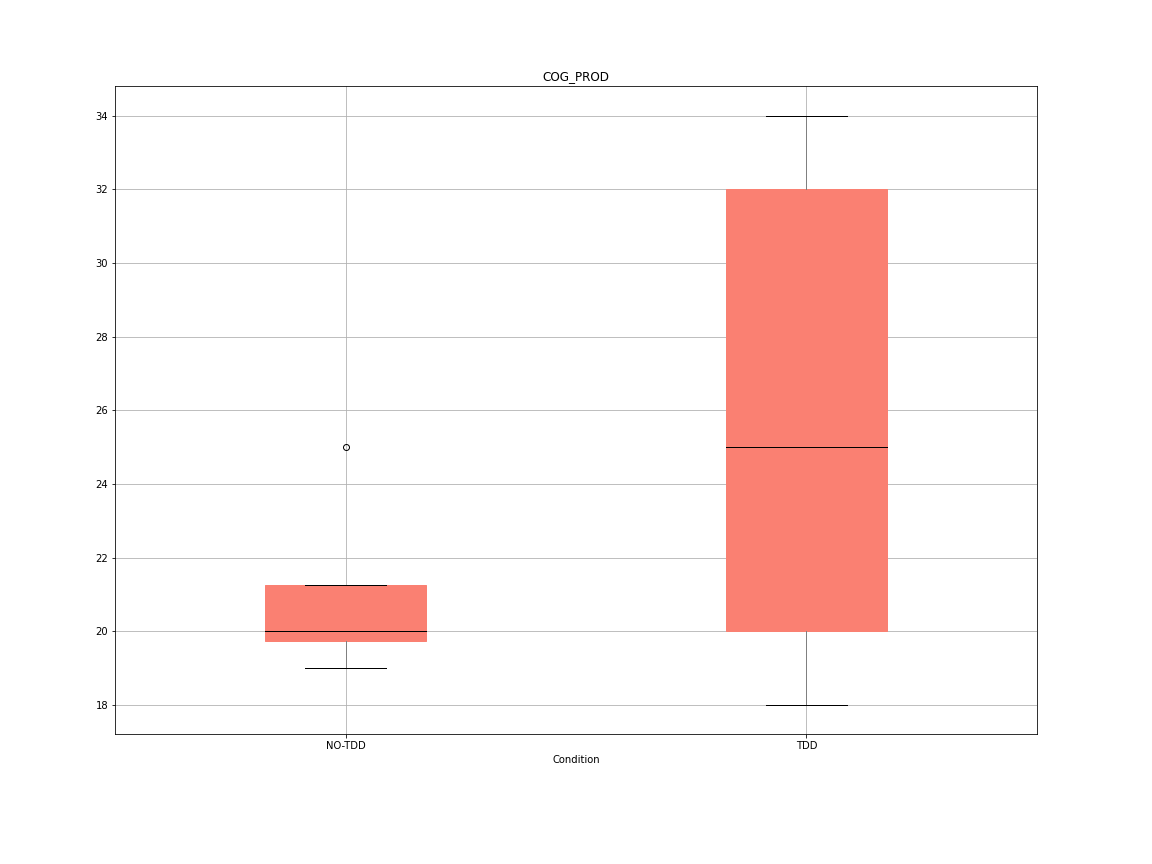
\includegraphics[width=\linewidth]{figures/box_plots/task3/COG.png}
        \caption{COG}
        \label{bp_task3_cog}
    \end{subfigure}\hfil
    \begin{subfigure}{0.33\textwidth}
        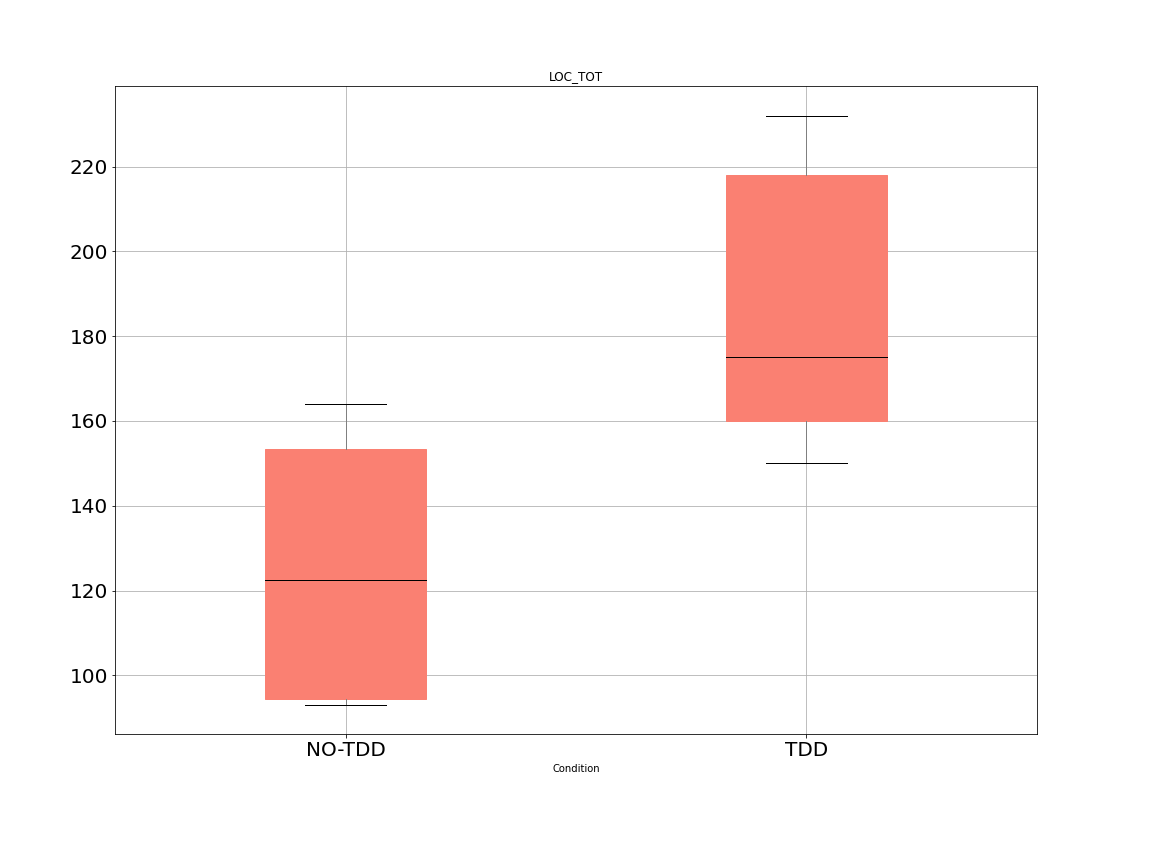
\includegraphics[width=\linewidth]{figures/box_plots/task3/LOC.png}
        \caption{LOC}
        \label{bp_task3_loc}
    \end{subfigure}
    \caption{Box plot charts for \textit{Exp2}.}
    \label{box_plots_task3}
\end{figure}

\ \\ \
Let's now consider both \textit{Exp1} and \textit{Exp2} simultaneously. As for $QLTY$, the comparison between \tdd and \notdd seems in favor of the former for any experimental task; indeed, by looking at table \ref{tab_dv_t1_2}  and figures \ref{box_plots_task1_2}.a - which aggregate the results for both tasks in \textit{Exp1} - and \ref{box_plots_task3}.a, we can notice how the boxes for \tdd in the charts are higher than, or comparable to the ones for \notdd. The same trend is confirmed by the mean and median values (see table \ref{tab_dv_t1_2}). However, we can notice that the effect of \tdd on $QLTY$ is not uniform across the experimental tasks: the gap between \tdd and \notdd is wider for the experimental task in \textit{Exp2}, while it is more limited for the two
experimental tasks in \textit{Exp1}.

As for $PROD$, it seems that the effect of \tdd is contrasting across the experimental tasks; in particular, when considering the first task in \textit{Exp1} and the one in \textit{Exp2}, the boxes for \tdd are  higher than the
boxes for \notdd (figures \ref{box_plots_task1}.b and \ref{box_plots_task3}.b). On the contrary, the box for \tdd is lower than the one for \notdd in the second experimental task of \textit{Exp1} (figures \ref{box_plots_task2}.b and \ref{box_plots_task3}.b). Such a contrasting trend is confirmed when looking at the mean and median values (see table \ref{tab_dv_t1_2}).

Finally, if we consider the number of test cases written by the participants (\ie the $TEST$ dependent variable), we can see how - similarly to the $QLTY$ variable  (see figures \ref{box_plots_task1_2}.c and \ref{box_plots_task3}.c) - the boxes for \tdd are either higher than or comparable to the ones for \notdd. Moreover, the median values for both experiments are still higher for \tdd, while the majority of values in the boxes are close together, especially in \textit{Exp2}.


\begin{table}[H]
    \begin{center} 
        \begin{tabular}{ |p{2cm}||p{1.6cm}|p{1.6cm}|p{1.6cm}|p{1.6cm}|p{1.6cm}|}
            \hline
                \multicolumn{6}{|c|}{\textit{Exp1} - TDD} \\
            \hline
                Metric & Min & Max & Mean & Median & Std\\
            \hline
                QLTY & 50 & 100 & 82.97 & 82 & 17.43 \\
                PROD & 8 & 100 & 58.33 & 72 & 35.76 \\
                TEST & 0 & 13 & 7.22 & 8 & 4.26 \\
                CYC & 9 & 28 & 17.66 & 19 & 7.51 \\
                COG & 2 & 40 & 15.55 & 14 & 12.06 \\
                LOC & 80 & 203 & 145.33 & 154 & 39.97 \\
            \hline\hline
                \multicolumn{6}{|c|}{\textit{Exp1} - NO-TDD} \\
            \hline
                Metric & Min & Max & Mean & Median & Std\\
            \hline
                QLTY & 65.55 & 94.43 & 78.78 & 78.77 & 9.11 \\
                PROD & 52 & 84 & 69.11 & 73 & 13.22 \\
                TEST & 0 & 12 & 6.11 & 7.0 & 5.08 \\
                CYC & 12 & 36 & 19.11 & 16 & 7.07 \\
                COG & 9 & 49 & 20.66 & 15 & 12.56 \\
                LOC & 74 & 260 & 154.22 & 157 & 60.32 \\
            \hline
            \hline
                \multicolumn{6}{|c|}{\textit{Exp2} - TDD} \\
            \hline
                Metric & Min & Max & Mean & Median & Std\\
            \hline
                QLTY & 85 & 100 & 95 & 100 & 7.07 \\
                PROD & 83.33 & 100 & 93.33 & 100 & 9.13 \\
                TEST & 7 & 18 & 11.6 & 12 & 4.15 \\
                CYC & 15 & 30 & 22.6 & 20 & 6.58 \\
                COG & 18 & 34 & 25.8 & 25 & 7.08 \\
                LOC & 150 & 232 & 187 & 175 & 36.15 \\
            \hline\hline
                \multicolumn{6}{|c|}{\textit{Exp2} - NO-TDD} \\
            \hline
                Metric & Min & Max & Mean & Median & Std\\
            \hline
                QLTY & 80 & 100 & 86.25 & 82.5 & 9.46 \\
                PROD & 75 & 100 & 83.33 & 79.16 & 11.78 \\
                TEST & 0 & 11 & 4.5 & 3.5 & 5.44 \\
                CYC & 16 & 23 & 19.5 & 19.5 & 2.88 \\
                COG & 19 & 25 & 21 & 20 & 2.70 \\
                LOC & 93 & 164 & 125.5 & 122.5 & 36.82 \\
            \hline
        \end{tabular}
        \caption{\label{tab_dv_t1_2}Dependent variables' statistics for \textit{Exp1} and \textit{Exp2}.}
    \end{center}
\end{table}



\subsection{Meta-analysis}
Figure \ref{fp_qlty_prod} displays the results of the aggregate analysis on the variables for \textit{Exp1} and \textit{Exp2} through means of forest plot charts, focusing on the $QLTY$ and $PROD$ variables.
The SMDs relative to the $QLTY$ variable for the single experiments (see figure \ref{fp_qlty_prod}.a) are both in favor of \tdd; in particular, the SMD is considered small (0.290) in \textit{Exp1} and large (0.950) in \textit{Exp2}, highlighting how the effect of \tdd on $QLTY$ is not uniform and may depend on the tackled task; the overall SMD is still in favor of \tdd and small (0.480).

\begin{figure}[H]
    \begin{subfigure}{0.49\textwidth}
        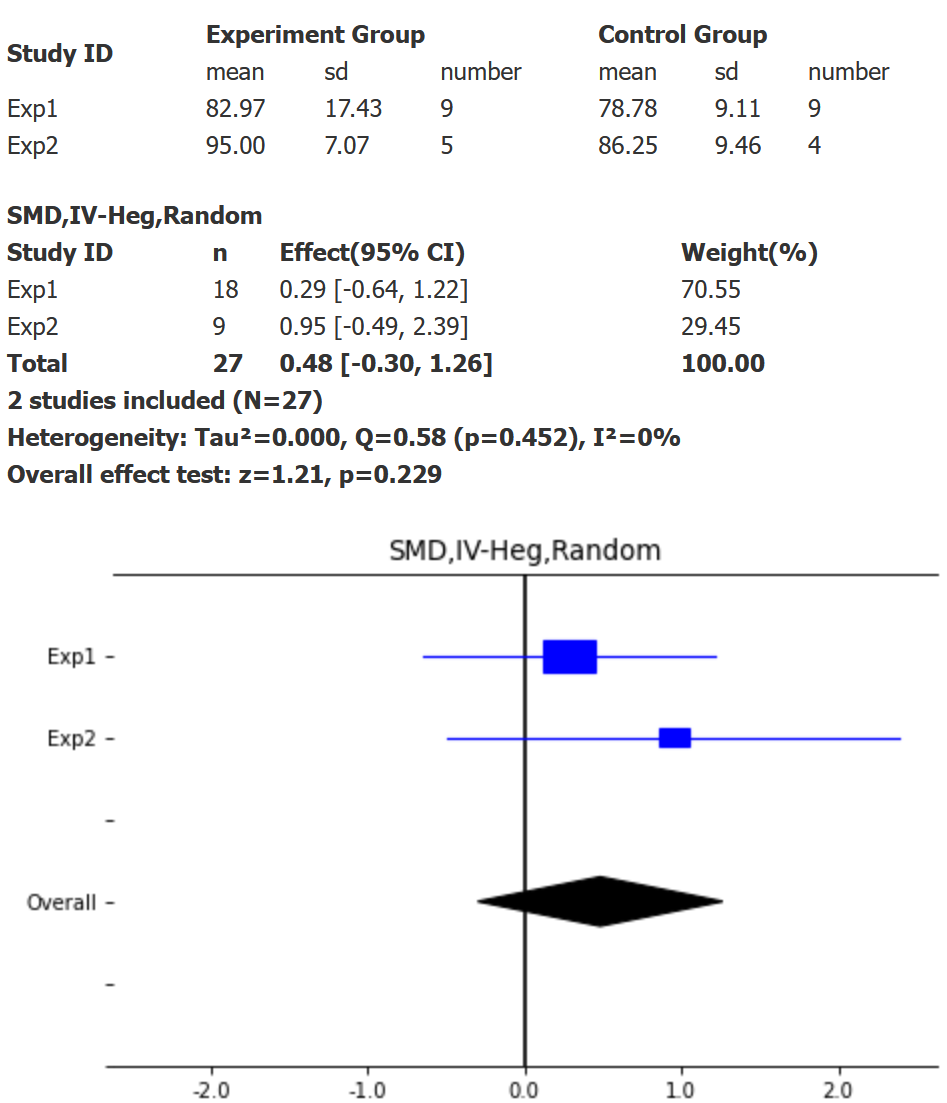
\includegraphics[width=\linewidth]{figures/forest_plots/QLTY.png}
        \caption{QLTY}
        \label{fp_qlty}
    \end{subfigure}\hfil
    \begin{subfigure}{0.49\textwidth}
        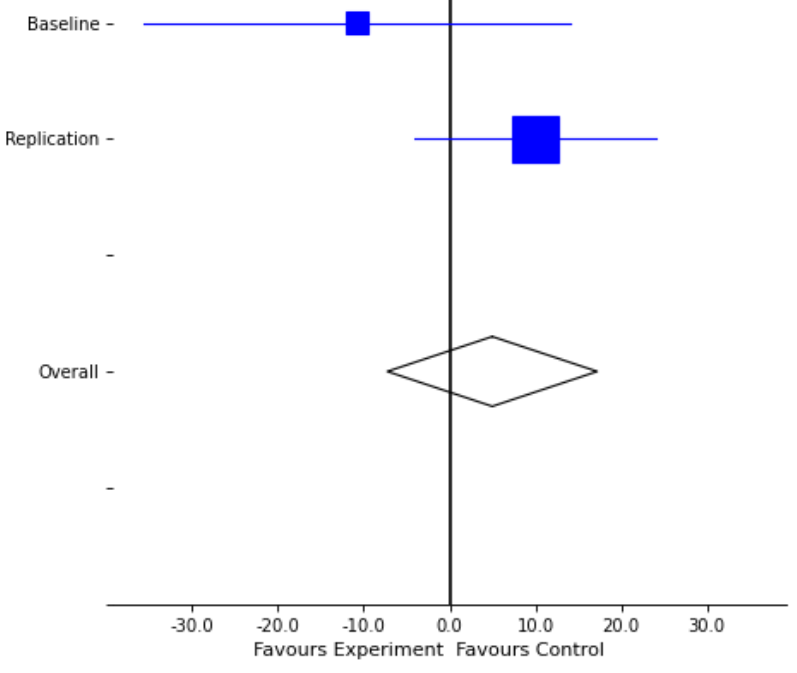
\includegraphics[width=\linewidth]{figures/forest_plots/PROD.png}
        \caption{PROD}
        \label{fp_prod}
    \end{subfigure}
    \caption{Forest plot charts for the $QLTY$ and $PROD$ variables.}
    \label{fp_qlty_prod}
\end{figure}

Figure \ref{fp_qlty_prod}.b displays the forest plot for the $PROD$ variable. Here, the SMD for \textit{Exp1} is in favor of \notdd and small (-0.380); this is due to the second experimental task, as expected from looking at the box plots charts in figure \ref{box_plots_task2}. For \textit{Exp2}, on the other hand, the SMD is in favor of \tdd and large (0.860). The joint SMD is still in favor of \tdd but is negligible (0.120); the hollow joint SMD indicates a higher heterogeneity ($I^2$ is more than 50\%).

Finally, figure \ref{fp_test} plots the results for the meta-analysis relative to the $TEST$ variable. Here, similarly to what happens with the $QLTY$ variable, both experiments are in favor of \tdd: the SMD for \textit{Exp1} is small (0.230), which is again expected given the contrast between the first two experimental tasks, while the SMD for \textit{Exp2} is large (1.330). The joint SMD is still in favor of \tdd and medium (0.600).

\begin{figure}[H]
    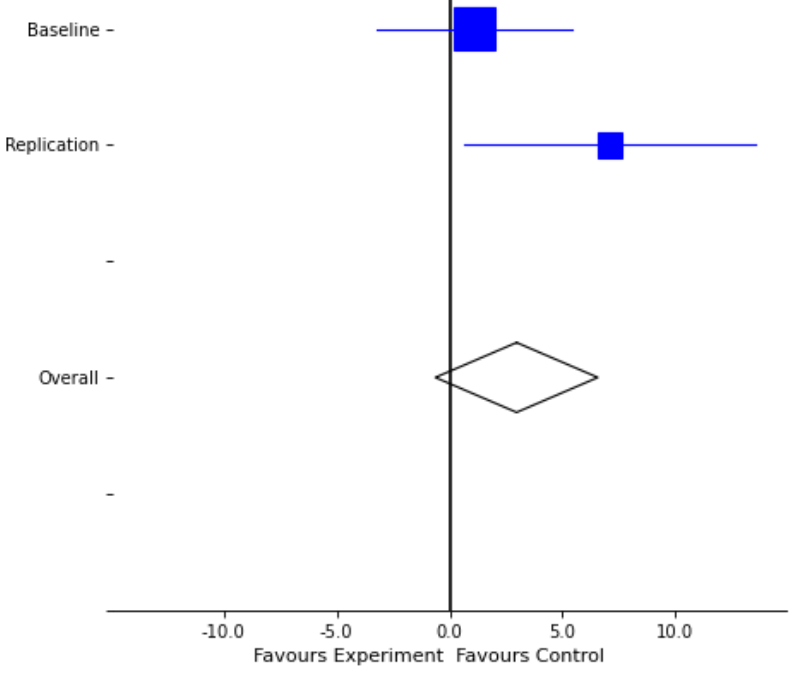
\includegraphics[width=\linewidth]{figures/forest_plots/TEST.png}
    \caption{Forest plot chart for the $TEST$ variable.}
    \label{fp_test}
\end{figure}\hfil
    
Given that for all three variables, the 95\% CI interval contains the 0, and especially considering the small size of this study, the meta-analysis alone does not indicate a statistical significance in favor of any of the two approaches for any of these variables.
A non-significant result does not mean that the treatment has no effect or that the difference is not meaningful; it simply means that there is not enough evidence to support a claim of a significant effect; therefore, we are in need of further replication to reach a statistical conclusion on the effects of \tdd on external quality, productivity, and number of tests.



\subsection{Post-questionnaire analysis}
Figure \ref{bar_charts} summarizes the answers provided by the participants in the post-experiment questionnaires submitted at the end of each task for \textit{Exp1}, comparing the responses by the employed approach (\tdd or \notdd).
Regarding user story comprehensibility, in the first experimental task, \textit{IO}, the participants had a similar level of agreement on the matter, with the majority finding the provided user stories easy or very easy. In the second task, \textit{CR}, there is a more substantial difference, with only 40\% of the \tdd group having a positive perception of the user stories' clarity, compared to the 87\% of the \notdd group.

As for the second question, regarding the feelings of the participants on the general task difficulty, in the first experimental task the participants somewhat agree, with 50\% of the \tdd group and 40\% of the \notdd group feeling neutral about the difficulty of the task; no one in the \tdd group found the task very easy, however, compared to a 20\% in the \notdd group. In the second task, the answers are quite in favor of \notdd, with 60\% of the \tdd group having some difficulties with the implementation of the provided user stories; 20\% however found the task very easy. On the other hand, all of the participants in the \notdd group agreed on feeling neutral about their ease in developing the task.

Finally, question three was focused on the difficulty of the participants in applying their reference condition: for task 1, the \tdd group did not have a strong opinion on applying this technique, with 75\% feeling neutral about it, and the other 25\% finding the application of \tdd easy but not too easy; as for the \notdd group, this had also the majority of opinions feeling neutral about their approach (60\%), however this time 20\% of the participants felt very good about applying \notdd; this is probably due to them being overall more accustomed to the approach. This conveys the idea that \tdd was considered less easy to apply compared to \notdd; such a trend is even clearer when considering the second experimental task, where 80\% of the \tdd group had trouble with their approach(40\% answered ``Very Hard" and 40\% answered ``Hard"), compared to only 25\% for the participants that used \notdd.


\begin{figure}[htbp]
    \begin{subfigure}{\textwidth}
        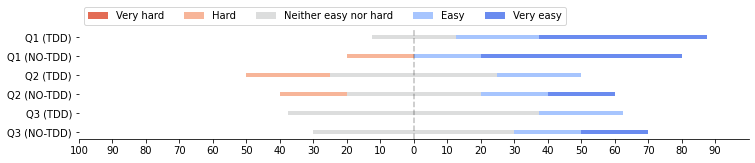
\includegraphics[width=\textwidth]{figures/bar_charts/task1.png}
        \caption{First task for \textit{Exp1}, \textit{IO}.}
    \end{subfigure}
    
    \bigskip
    
    \begin{subfigure}{\textwidth}
        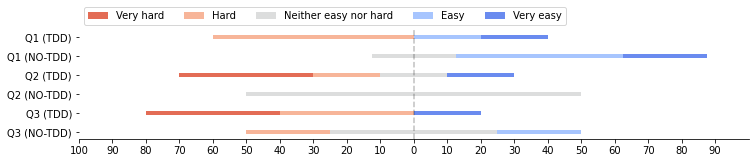
\includegraphics[width=\textwidth]{figures/bar_charts/task2.png}
        \caption{Second task for \textit{Exp1}, \textit{CR}.}
    \end{subfigure}
    
    \caption{Diverging stacked bar charts for the post-questionnaires.}
    \label{bar_charts}
\end{figure}

\newpage
Moving to the open-ended questions, we performed thematic analysis in order to identify a base template on which to parse the answers provided by the participants in the same post-questionnaires.
The themes we identified are:

\begin{enumerate}
    \item General feelings on the development task.
    \item Feelings on \tdd and \notdd to accomplish the task.
    \item \notdd testing approach.
    \item Personal comparison and thoughts between \tdd and \notdd.
\end{enumerate}

Most of the participants found the first development task easy, with 6 out of 9 expressing a positive feeling about it; 2 out of the remaining 3 found some challenges and would have liked a bit more time, while the last participant did not answer. 
For the second task, 2 out of 9 students had no issues with it, while 6 found the task to be harder than the previous one: out of the latter, 3 reported struggling with implementing some user stories, while the other 3 simply stated that the task was more challenging, without voicing in detail their struggles with it.


Employing \tdd to tackle the tasks was still not fully clear at the end of \textit{Exp1}: for task 1, 2 participants expressed how getting into the \tdd mindset for a new problem was not so easy for them, while another student, participant 2, found this practice very useful and expressed their good feelings for having learned it:
\begin{mdframed}
    \textit{``I think TDD is very helpful, and I am glad that I can learn it."}
\end{mdframed}


In the second task, which as we have seen in the interval-scale questions was considered overall harder, 3 out of 5 participants in the \tdd group expressed having trouble with it.
For example, participants 5 stated:
\begin{mdframed}
    \textit{``I think the CleaningRobot was harder than the IntelligentOffice, but maybe only because of \tdd."}
\end{mdframed}

While expressing a similar feeling, participant 8 also said how more experience with \tdd would be beneficial to them:
\begin{mdframed}
    \textit{``It is hard to think the other way around as a software developer, but I think in my opinion \tdd is very useful and if you are used to it, it can really help you a lot to improve your programming."}
\end{mdframed}

Out of the \notdd group, on the other hand, the majority had no particular issue with the approach in both tasks.
However, in the post-questionnaire for \textit{CR} 2 participants expressed how in their opinion, since this task was harder, maybe employing \tdd would have made it easier, since it would have allowed them to tackle the user stories in a more incremental manner; for example, participant 3 said:
\begin{mdframed}
    \textit{``With \tdd I wouldn't have fallen into some pitfalls; I had to rewrite some code because I didn't know I broke some components with features that I added later. With \tdd I would have known way earlier."}
\end{mdframed}

As for the chosen \notdd approach, in the first task, 3 out 5 participants dealing with this testing approach still wrote test cases after the production code, while the other 2 chose not to; for the second task, all 4 participants in the \notdd group tested their implementation, which is in line with them finding \textit{CR} overall harder.

At the end of the second task, 4 participants expressed their preference with \tdd, while 3 were still more comfortable with \notdd. Finally, one participant stated how in their opinion the best approach to use depends on how refined the requirements for the task to implement are, stating how they would prefer \tdd, but only if the functional requirements are clear, while for discovering new technologies, they wouldn't use \tdd for sure:
\begin{mdframed}
    \textit{``\tdd reduces bugs, if you break something with a refactoring you know it instantly, and the tests are like documentation. With \notdd bugs and functional errors are only known at the end of the testing phase, which for me is terrible. I would now prefer \tdd, but only if the functional requirements are clear. For discovering technology, I wouldn't use \tdd for sure."}
\end{mdframed}



\subsection{Final interview analysis}
Thematic analysis was also used to extract patterns from the final individual participant interviews; we identified the following main topics: 
\begin{enumerate}
    \item Thoughts on the replication experiment.
    \item Refactoring with \tdd.
    \item \notdd testing approach.
    \item Applying \tdd for \ess development.
    \item Prior participant testing experience.
    \item Thoughts on the overall experience with the studies, from the lectures and homework, to the last development task.
\end{enumerate}

For the first point, 5 out of 9 participants found the task straight forward and had no issues with its development, while the other 4 found it balanced, with some user stories requiring more thought before being implemented, according to them. Furthermore, 3 participants stated how they were already familiar with some of the sensors and actuators used for the task, either from previous university courses, or from personal experience.

As a reminder, for \textit{Exp2}, 5 out of 9 participants were (randomly) assigned the \tdd version, while the other 4 had to develop the \es using \notdd; out of the 5 that used \tdd, 4 of them performed some minor refactoring, either in the test cases or in the production code, while 1 did not.
As for the \notdd group, half still wrote tests (although many less compared to the \tdd group, as we have seen from the gathered data) after implementing the user stories, while the other half did not.

When discussing the employment of \tdd and \notdd in the context of \ess and their strengths and weaknesses, some participants expressed how they were not comfortable providing a definitive answer on the matter, mostly given their still limited experience with \tdd. Others conveyed how the best approach depends on the task they are working on, similarly to what happened in the post-questionnaire for \textit{CR}; for example, participant 7 said:
\begin{mdframed}
    \textit{``The task (SR) was pretty easy for me; as a result I think that \tdd was not really needed [...], it was a bit overkill. On the second task (CR), however, which I found much more complex, I feel like TDD was much more beneficial."}
\end{mdframed}

Participants also provided information about their testing experience prior to the study: 2 of them had no testing experience at all; on the other hand, 4 students already had some unit testing experience, while 3 had limited and mostly theoretical knowledge of \tdd, obtained in a previous university course.
Concerning the learning experience with \tdd, while some participants expressed how at the end of the study they were still more comfortable using \notdd, one of the students among those with no prior testing, experience stated:
\begin{mdframed}
\textit{``I had no prior testing experience at all, so it was very nice to learn about it in the lectures, especially \tdd; I would use \tdd for sure going forward, especially with even more experience. The main challenge was getting into it in the beginning."}
\end{mdframed}

Considering the last point, most students appreciated the overall experience and expressed how they enjoyed the mixture of theory and practice on \tdd and the other concepts explored. For example, participant 4 (\tdd) stated:
\begin{mdframed}
    \textit{``I enjoyed the overall experience made up of a mix of theory and practical stuff."}
\end{mdframed}

Something very interesting that came up during the thematic analysis of these interviews, especially from the lecturer's point of view, is that participants expressed a high interest into the hardware deployment step: 5 out of the 9 students that have been interviewed, in fact, demonstrated genuine interest in seeing their developed \es in action, making use of real sensors and actuators and operating on a real hardware platform. 
Participants 2 and 3, for example, stated:
\begin{mdframed}
    \textit{``Nice to see it run and test by yourself with hardware and with the sensors."}
\end{mdframed}
\begin{mdframed}
    \textit{``I knew most of the sensors so developing this task was not hard for me, but still really cool to implement because I wanted to see it in action on real hardware."}
\end{mdframed}

Keep in mind that there was no reference to this aspect in the script for the interview, so each of the participants that showed interest in the topic, did so out of their initiative while discussing their thoughts on this task; also, each student was alone during their interview, so it is unlikely that the answers were influenced by each other.


